\documentclass[a4paper]{article}

\usepackage[utf8]{inputenc}
\usepackage[english]{babel}
\usepackage[T1]{fontenc}
\usepackage[margin=2cm]{geometry}

\usepackage{tikz}

\usepackage{float}

\usepackage{amsmath}
\usepackage{amsfonts}
\usepackage{amsthm}
\usepackage{amssymb}
\usepackage{thmtools}
\usepackage{mathrsfs}

\usepackage{enumitem}

\usepackage{chngcntr}
\counterwithin{figure}{subsection}

\makeatletter
\def\th@mytheorem{
  \thm@notefont{}
}
\makeatother

\theoremstyle{mytheorem}

\newtheorem{definition}{Definition}[section]
\newtheorem{remark}[definition]{Remark}
\newtheorem{property}[definition]{Property}
\newtheorem{theorem}[definition]{Theorem}
\newtheorem{conjecture}[definition]{Conjecture}
\newtheorem{lemma}[definition]{Lemma}

\setitemize[1]{label=\textbullet}
\setitemize[2]{label=$\circ$}

\DeclareMathOperator{\rank}{rank}
\DeclareMathOperator{\id}{id}

\begin{document}

Synthesis of~\cite{highestRankOfAn},~\cite{A12PolytopesRank},~\cite{highRankAlternating},~\cite{bookIncidenceGeometry} and~\cite{cprGraph}.

\section{Abstract Polytopes}

\begin{definition}[Partially ordered set]
  A \textit{partially ordered set} is a pair $(R,\le)$ with $R$ a set and $\le$ a relation between $R$ and $R$ such that
  \begin{enumerate}
    \item $F \le F$ ($F \in R$)
    \item if $F \le G$ and $G \le F$, we have $F=G$ ($F,G \in R$)
    \item if $F \le G$ and $G \le H$, we have $F \le H$ ($F,G,H \in R$)
  \end{enumerate}
\end{definition}

\begin{definition}[Face of a partially ordered set]
  In the context of abstract polytopes, we denote elements of the poset, \textit{faces}.
\end{definition}

\begin{definition}[Ranked partially ordered set]
  A poset is ranked if there exists a function $\rank : R \to \mathbb Z$ such that
  \begin{enumerate}
    \item if $F < G$, then $\rank(F) < \rank(G)$ $(F, G \in R)$
    \item if $F < G$ and there exists no $H \in R$ such that $F < H < G$, then $\rank(G) = \rank(F) + 1$ $(F, G \in R)$.
  \end{enumerate}
\end{definition}

\begin{definition}[$i$-face]
  If a face have a rank equals to $i$, we will call this face a $i$-face.
\end{definition}

\begin{definition}[Totally ordered set]
  A \textit{totally ordered set} is a poset such that $\forall x,y \in R$, we have $x \le y$ or $y \le x$.
\end{definition}

\begin{definition}[Flag of a partially ordered set]
  A \textit{flag} of a partially ordered set is a maximal totally ordered which is a subset of the poset.
\end{definition}

\begin{definition}[Abstract $d$-polytope]
  An \textit{abstract $d$-polytope} $\mathcal P$ is a ranked partially ordered set of \textit{faces}. Such that
  \begin{enumerate}
    \item $\mathcal P$ contains two improper faces, a least face $F_{-1}$ and a greatest face $F_d$.
    \item The flags of $\mathcal P$ contains $d + 2$ faces (includind the 2 improper faces)
    \item $\mathcal P$ is strongly connected (see below)
    \item Let $F, G$ be two faces of $\mathcal P$ such that $\rank(F) = i - 1$ and $\rank(G) = i + 1$. Then there exists exactly 2 $i$-faces $H$ such that $F < H < G$. This is called the diamond property.
  \end{enumerate}
\end{definition}

\begin{definition}[Section of a poset]
  For any two faces $F, G$ with $F \le G$, we define the \textit{section} \[
    F/G = \{H | H \in R, F \le H \le G\}
  \]
\end{definition}

\begin{property}
  Every section of a polytope is a polytope
\end{property}

\begin{definition}[Connected poset]
  A poset which satisfy the two first properties of a polytope is said \textit{connected} if $d \le 1$ or if, for any proper faces $F, G$, there exists a sequence of proper faces $F = H_0, H_1, \dots, H_{k-1}, H_k = G$. such that $H_i$ and $H_{i+1}$ are compararable for every $i$.
\end{definition}

\begin{definition}[Strictly connected poset]
  A poset is \textit{strictly connected} if every section (including the whole poset) is connected.
\end{definition}

\begin{definition}[Adjacent flags]
  Two flags of a $d$-polytope are said adjacent if they differ by exactly one face.
\end{definition}

\begin{definition}[$i$-adjactent flag]
  Let $\Phi$ be a flag, we know by the diamond property that there exists exactly a flag that share all faces execpt the face of rank $i$ with $\Phi$. We call this face the $i$-adjacent flag of $\Phi$ and we denote it $\Phi^i$.
\end{definition}

\begin{property}
  \[
    \left(\Phi^i\right)^i = \Phi
  \]
\end{property}

\begin{property}
  \[
    \left(\Phi^i\right)^j = \left(\Phi^j\right)^i \quad \text{if} \ |i-j| > 1.
  \]
\end{property}

\begin{definition}[Equivar polytope]
  A $d$-polytope is said \textit{equivar} if for all $i = 1, 2, \dots, d-1$ there is an integer $p_i$ such that any section $G/F$ where $F$ is $(i-2)$-face and $G$ is a $(i+1)$-face.
\end{definition}

\begin{definition}[Schläfli type]
  If $\mathcal P$ is equivelar, we say that ha have a \textit{Schläfli type} of $\{p_1, \dots, p_{d-1}\}$.
\end{definition}

\begin{definition}[Regular polytope]
  A polytope is regular if it's automoprhism group have exactly one orbit over the flags.
\end{definition}

\begin{property}
  Equivalently, a polytope is regular if for some flag $\Phi$, and each $i$, there exists a unique involutory automorphism $\rho_i$ such that $\Phi_i = \Phi \rho_i$. In fact this property holds for every flag.
\end{property}

\begin{definition}[Base flag]
  We choose a fixed flag of a polytope and we call it the \textit{base flag}.
\end{definition}

\begin{property}
  For a regular $d$-polytope with base flag $\Phi$, it's group $\Gamma(\Phi)$ is generated by the involutions $\rho_i$ defined below.
\end{property}

\begin{definition}[Distinguised generator]
  The $\rho_i$ are called the \textit{distinguished generators}.
\end{definition}

\section{Groups}

\begin{definition}[String group generated by involutions]
  Let $G$ be a group and $S = \{\rho_0, \dots, \rho_n\}$ be a set of involutions which generate $G$ such that
  \begin{center}
    $\forall i,j$ with $| i - j| > 1$ $\rho_i$ and $\rho_j$ commute.
  \end{center}
  We call the pair $(G,S)$ a \textit{string group generated by involutions}
\end{definition}

\begin{definition}[string C-group]
  Denote $\Gamma_I$ the group generated by $\{\rho_i : i \in I\}$ where $I \subseteq \{0\dots r-1\}$. A sggi $(G,S)$ is a \textit{string C-group} if it satisfies the intersection property:
  \begin{center}
    $\Gamma_I \cap \Gamma_J = \Gamma_{I \cap J}$ where $I, J \subseteq \{0\dots r-1\}$. We denote $\Gamma = (G,S)$ for string C-groups.
  \end{center}
\end{definition}

\begin{definition}[Rank of a string C-group]
  The \textit{rank of a string C-group} $\Gamma = (G,S)$ is $|S|$.
\end{definition}

\begin{remark}[Group $\Gamma$]
  We will talk about the group $\Gamma$ where $\Gamma = (G,S)$ to talk about the group $G$.
\end{remark}

\begin{remark}[Rank of $G$]
  We will talk about the rank of the group $G$ as the maximum size of a set $S$ of involutions such that $\Gamma = (G,S)$.
\end{remark}

\begin{property}
  The group of automorphisme of a regular polytope and the distinguished generators forms a string C-group and the Schälfli symbol of this polytope is $\{p_1, \dots, p_d\}$
\end{property}

\begin{property}
  A $d$-polytope can be uniquely constructed from a string $C$-group.
\end{property}

\section{Properties of groups}

\begin{property}
  Let $\Gamma = \langle \rho_0, \dots, \rho_{r-1} \rangle$ be a sggi such that $\Gamma_0, \Gamma_{r-1}$ are string C-groups and $\Gamma_0 \cap \Gamma_{r-1} = \Gamma_{0,r-1}$ then $\Gamma$ is a string C-group.
\end{property}

\begin{property}
  Let $\Gamma$ be a sggi, if $\Gamma_0$ and $\Gamma_{r-1}$ are string C-group, $\rho_{r-1} \notin \Gamma_{r-1}$ and $\Gamma_0$ is maximal
\end{property}

\cleardoublepage{}

\section{Premier jet}

\begin{conjecture}
  Let $H$ be a string C-group generated by involutions $\rho_1, \dots, \rho_{r-1}$ such that $H$ fixes exactly 2 points. Then this string C-group can not be extended to a transitive group $G$, generated by involutions $\rho_0, \dots, \rho_{r-1}$ if $G$ only contains even permutations.
\end{conjecture}

\begin{proof}
  Here are some counter-examples (involution added in $G$ is dashed):
  \begin{center}
    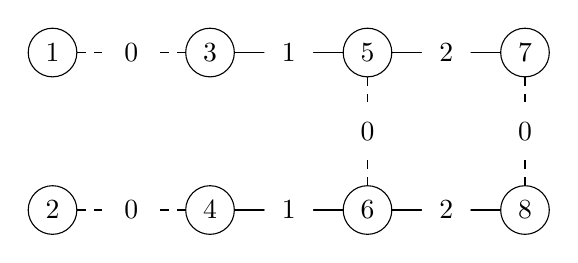
\begin{tikzpicture}

      \begin{scope}[every node/.style={circle,draw}]
        \node (1) at (0,2) {1};
        \node (2) at (0,0) {2};
        \node (3) at (2,2) {3};
        \node (4) at (2,0) {4};
        \node (5) at (4,2) {5};
        \node (6) at (4,0) {6};
        \node (7) at (6,2) {7};
        \node (8) at (6,0) {8};
      \end{scope}

      \begin{scope}[every node/.style={fill=white,circle}]

        \begin{scope}[every edge/.style={draw}]
          \path (3) edge node {$1$} (5);
          \path (4) edge node {$1$} (6);
          \path (5) edge node {$2$} (7);
          \path (6) edge node {$2$} (8);
        \end{scope}

        \begin{scope}[every edge/.style={draw,dashed}]
          \path (1) edge node {$0$} (3);
          \path (2) edge node {$0$} (4);
          \path (5) edge node {$0$} (6);
          \path (7) edge node {$0$} (8);
        \end{scope}

      \end{scope}

    \end{tikzpicture}
  \end{center}

  \begin{center}
    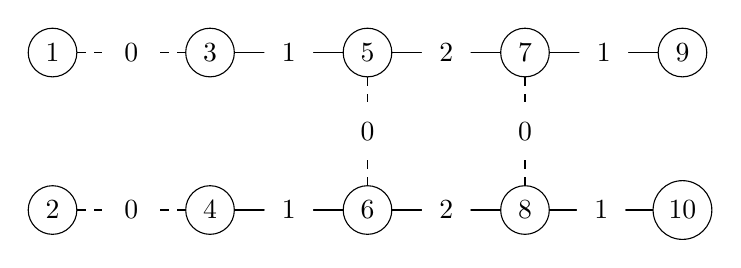
\begin{tikzpicture}

      \begin{scope}[every node/.style={circle,draw}]
        \node (1)  at (0,2)  {1};
        \node (2)  at (0,0)  {2};
        \node (3)  at (2,2)  {3};
        \node (4)  at (2,0)  {4};
        \node (5)  at (4,2)  {5};
        \node (6)  at (4,0)  {6};
        \node (7)  at (6,2)  {7};
        \node (8)  at (6,0)  {8};
        \node (9)  at (8,2)  {9};
        \node (10) at (8,0)  {10};
      \end{scope}

      \begin{scope}[every node/.style={fill=white,circle}]

        \begin{scope}[every edge/.style={draw}]
          \path (3)  edge node {$1$} (5);
          \path (4)  edge node {$1$} (6);
          \path (5)  edge node {$2$} (7);
          \path (6)  edge node {$2$} (8);
          \path (7)  edge node {$1$} (9);
          \path (8)  edge node {$1$} (10);
        \end{scope}

        \begin{scope}[every edge/.style={draw,dashed}]
          \path (1)  edge node {$0$} (3);
          \path (2)  edge node {$0$} (4);
          \path (5)  edge node {$0$} (6);
          \path (7)  edge node {$0$} (8);
        \end{scope}

      \end{scope}

    \end{tikzpicture}
  \end{center}

  \begin{center}
    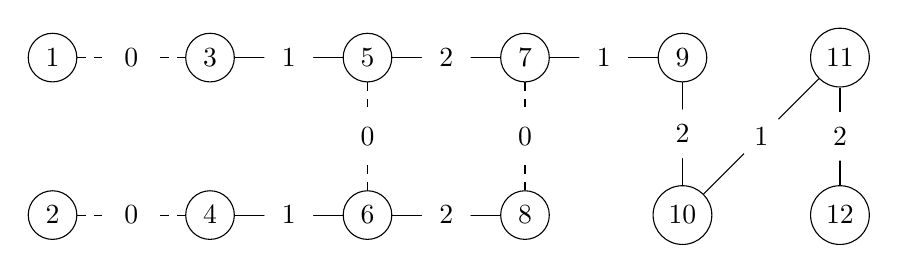
\begin{tikzpicture}

      \begin{scope}[every node/.style={circle,draw}]
        \node (1)  at (0,2)  {1};
        \node (2)  at (0,0)  {2};
        \node (3)  at (2,2)  {3};
        \node (4)  at (2,0)  {4};
        \node (5)  at (4,2)  {5};
        \node (6)  at (4,0)  {6};
        \node (7)  at (6,2)  {7};
        \node (8)  at (6,0)  {8};
        \node (9)  at (8,2)  {9};
        \node (10) at (8,0)  {10};
        \node (11)  at (10,2) {11};
        \node (12) at (10,0) {12};
      \end{scope}

      \begin{scope}[every node/.style={fill=white,circle}]

        \begin{scope}[every edge/.style={draw}]
          \path (3)  edge node {$1$} (5);
          \path (4)  edge node {$1$} (6);
          \path (5)  edge node {$2$} (7);
          \path (6)  edge node {$2$} (8);
          \path (7)  edge node {$1$} (9);
          \path (9)  edge node {$2$} (10);
          \path (10) edge node {$1$} (11);
          \path (11) edge node {$2$} (12);
        \end{scope}

        \begin{scope}[every edge/.style={draw,dashed}]
          \path (1)  edge node {$0$} (3);
          \path (2)  edge node {$0$} (4);
          \path (5)  edge node {$0$} (6);
          \path (7)  edge node {$0$} (8);
        \end{scope}

      \end{scope}

    \end{tikzpicture}
  \end{center}

  \begin{center}
    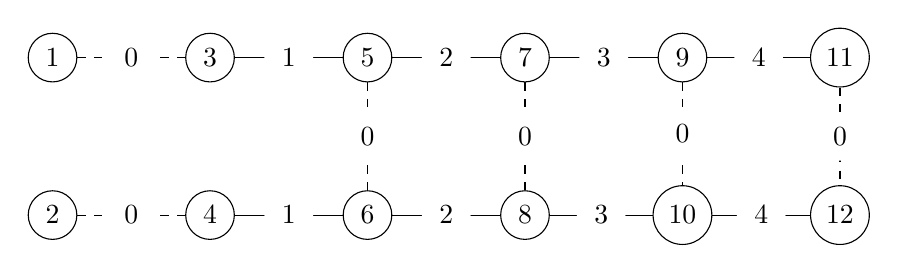
\begin{tikzpicture}

      \begin{scope}[every node/.style={circle,draw}]
        \node (1)  at (0,2)  {1};
        \node (2)  at (0,0)  {2};
        \node (3)  at (2,2)  {3};
        \node (4)  at (2,0)  {4};
        \node (5)  at (4,2)  {5};
        \node (6)  at (4,0)  {6};
        \node (7)  at (6,2)  {7};
        \node (8)  at (6,0)  {8};
        \node (9)  at (8,2)  {9};
        \node (10) at (8,0)  {10};
        \node (11) at (10,2) {11};
        \node (12) at (10,0) {12};
      \end{scope}

      \begin{scope}[every node/.style={fill=white,circle}]

        \begin{scope}[every edge/.style={draw}]
          \path (3)  edge node {$1$} (5);
          \path (4)  edge node {$1$} (6);
          \path (5)  edge node {$2$} (7);
          \path (6)  edge node {$2$} (8);
          \path (7)  edge node {$3$} (9);
          \path (8)  edge node {$3$} (10);
          \path (9)  edge node {$4$} (11);
          \path (10) edge node {$4$} (12);
        \end{scope}

        \begin{scope}[every edge/.style={draw,dashed}]
          \path (1)  edge node {$0$} (3);
          \path (2)  edge node {$0$} (4);
          \path (5)  edge node {$0$} (6);
          \path (7)  edge node {$0$} (8);
          \path (9)  edge node {$0$} (10);
          \path (11) edge node {$0$} (12);
        \end{scope}

      \end{scope}

    \end{tikzpicture}
  \end{center}

  \begin{center}
    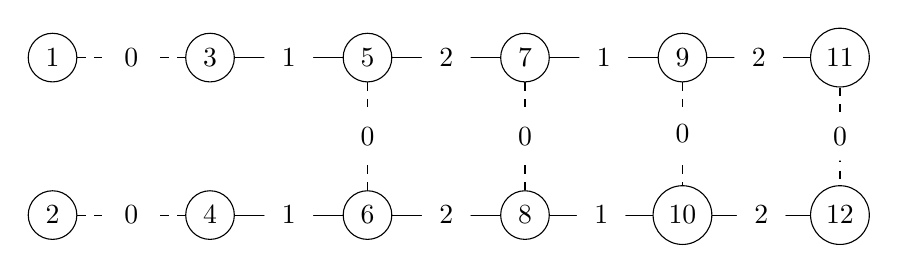
\begin{tikzpicture}

      \begin{scope}[every node/.style={circle,draw}]
        \node (1)  at (0,2)  {1};
        \node (2)  at (0,0)  {2};
        \node (3)  at (2,2)  {3};
        \node (4)  at (2,0)  {4};
        \node (5)  at (4,2)  {5};
        \node (6)  at (4,0)  {6};
        \node (7)  at (6,2)  {7};
        \node (8)  at (6,0)  {8};
        \node (9)  at (8,2)  {9};
        \node (10) at (8,0)  {10};
        \node (11) at (10,2) {11};
        \node (12) at (10,0) {12};
      \end{scope}

      \begin{scope}[every node/.style={fill=white,circle}]

        \begin{scope}[every edge/.style={draw}]
          \path (3)  edge node {$1$} (5);
          \path (4)  edge node {$1$} (6);
          \path (5)  edge node {$2$} (7);
          \path (6)  edge node {$2$} (8);
          \path (7)  edge node {$1$} (9);
          \path (8)  edge node {$1$} (10);
          \path (9)  edge node {$2$} (11);
          \path (10) edge node {$2$} (12);
        \end{scope}

        \begin{scope}[every edge/.style={draw,dashed}]
          \path (1)  edge node {$0$} (3);
          \path (2)  edge node {$0$} (4);
          \path (5)  edge node {$0$} (6);
          \path (7)  edge node {$0$} (8);
          \path (9)  edge node {$0$} (10);
          \path (11) edge node {$0$} (12);
        \end{scope}

      \end{scope}

    \end{tikzpicture}
  \end{center}

\end{proof}

\begin{conjecture}
  Let $H$ be a string C-group generated by involutions $\rho_1, \dots, \rho_{r-1}$ such that the degree of $H$ is odd and such that $H$ fixes exactly 2 points. Then this string C-group can not be extended to a transitive group $G$, generated by involutions $\rho_0, \dots, \rho_{r-1}$ if $G$ only contains even permutations.
\end{conjecture}

\begin{proof}
  \item
  \paragraph{}
  Nous allons prouver ceci par construction partons des points fixes de $H$, $1$ et $2$. On sait que ce sont des points fixes de $H$. Donc
  \begin{center}
    $1 \rho_i = 1$ et $2 \rho_i = 2$ pour $i \neq 0$.
  \end{center}

  \paragraph{}
  Vu que $G$ est transitif, il ne peut y avoir de points fixes et donc $1 \rho_0 \neq 1$ de même que $2 \rho_0 \neq 2$.

  \paragraph{}
  Si $ 1 \rho_0 = 2$ et donc $2 \rho_0 = 1$, on a une impossibilité car $G$ ne serait plus transitif. En effet l'orbite de $1$ ou $2$ serait $\{1,2\}$.

  \paragraph{}
  Donc $1 \rho_0 = 3$ et $2 \rho_0 = 4$ (nous choisissons les indices par simplicité).

  \paragraph{}
  Nous savons que $3$ et $4$ sont des points fixes par les involutions $\rho_i$ où $i \ge 2$. Sinon $(\rho_0\rho_i)^2 \neq 1$, vu que $1 \rho_i \neq 2$.

  \paragraph{}
  Si $3 \rho_1  = 4$, si $G$ est de degré $4$, alors il est transitif mais $\rho_1$ est une permutation impaire, ce qui ne satisfait pas à nos conditions.

  \paragraph{}
  Donc on a forcément $3 \rho_1 = 5$ et $4 \rho_1 = 6$, et on ne peut plus rajouter d'involutions sur les points $1, 2, 3, 4$. Au stade actuel, le graphe n'est pas encore transitif. On a le graphe suivant:

  \begin{center}
    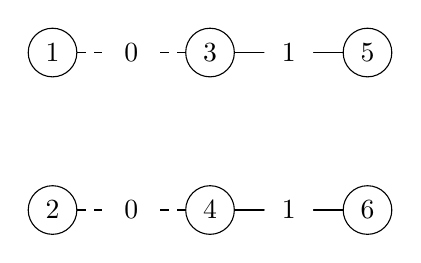
\begin{tikzpicture}

      \begin{scope}[every node/.style={circle,draw}]
        \node (1) at (0,2) {1};
        \node (2) at (0,0) {2};
        \node (3) at (2,2) {3};
        \node (4) at (2,0) {4};
        \node (5) at (4,2) {5};
        \node (6) at (4,0) {6};
      \end{scope}

      \begin{scope}[every node/.style={fill=white,circle}]

        \begin{scope}[every edge/.style={draw}]
          \path (3) edge node {$1$} (5);
          \path (4) edge node {$1$} (6);
        \end{scope}

        \begin{scope}[every edge/.style={draw,dashed}]
          \path (1) edge node {$0$} (3);
          \path (2) edge node {$0$} (4);
        \end{scope}

      \end{scope}

    \end{tikzpicture}
  \end{center}

  \paragraph{}
  On peut rajouter des arêtes entre 5 et 6 (pour rappel, on a prouvé qu'il était impossible de rajouter des arêtes sur 1, 2, 3 et 4). On peut dire que $\rho_0$ ou $\rho_2$ permutent 5 et 6. On trouve 3 graphes supplémentaires:

  \begin{center}
    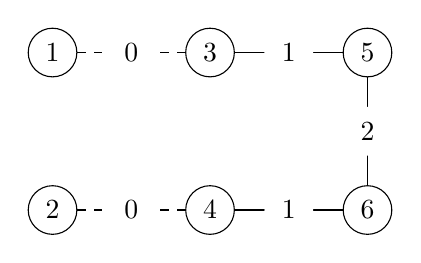
\begin{tikzpicture}

      \begin{scope}[every node/.style={circle,draw}]
        \node (1) at (0,2) {1};
        \node (2) at (0,0) {2};
        \node (3) at (2,2) {3};
        \node (4) at (2,0) {4};
        \node (5) at (4,2) {5};
        \node (6) at (4,0) {6};
      \end{scope}

      \begin{scope}[every node/.style={fill=white,circle}]

        \begin{scope}[every edge/.style={draw}]
          \path (3) edge node {$1$} (5);
          \path (4) edge node {$1$} (6);
          \path (5) edge node {$2$} (6);
        \end{scope}

        \begin{scope}[every edge/.style={draw,dashed}]
          \path (1) edge node {$0$} (3);
          \path (2) edge node {$0$} (4);
        \end{scope}

      \end{scope}

    \end{tikzpicture}
  \end{center}

  \begin{center}
    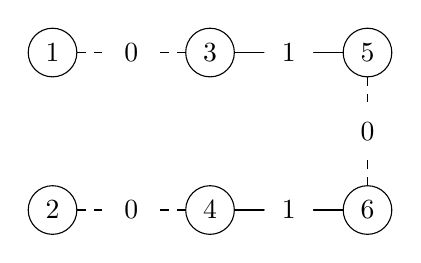
\begin{tikzpicture}

      \begin{scope}[every node/.style={circle,draw}]
        \node (1) at (0,2) {1};
        \node (2) at (0,0) {2};
        \node (3) at (2,2) {3};
        \node (4) at (2,0) {4};
        \node (5) at (4,2) {5};
        \node (6) at (4,0) {6};
      \end{scope}

      \begin{scope}[every node/.style={fill=white,circle}]

        \begin{scope}[every edge/.style={draw}]
          \path (3) edge node {$1$} (5);
          \path (4) edge node {$1$} (6);
        \end{scope}

        \begin{scope}[every edge/.style={draw,dashed}]
          \path (1) edge node {$0$} (3);
          \path (2) edge node {$0$} (4);
          \path (5) edge node {$0$} (6);
        \end{scope}

      \end{scope}

    \end{tikzpicture}
  \end{center}

  \begin{center}
    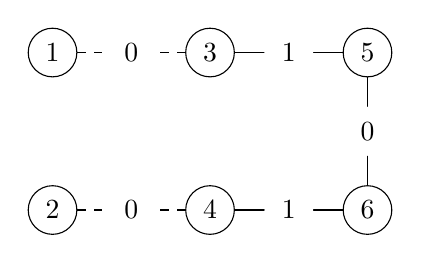
\begin{tikzpicture}

      \begin{scope}[every node/.style={circle,draw}]
        \node (1) at (0,2) {1};
        \node (2) at (0,0) {2};
        \node (3) at (2,2) {3};
        \node (4) at (2,0) {4};
        \node (5) at (4,2) {5};
        \node (6) at (4,0) {6};
      \end{scope}

      \begin{scope}[every node/.style={fill=white,circle}]

        \begin{scope}[every edge/.style={draw}]
          \path (3) edge node {$1$} (5);
          \path (4) edge node {$1$} (6);
          \path (5) edge node {$2$} (6);
        \end{scope}

        \begin{scope}[every edge/.style={draw,dashed}]
          \path (1) edge node {$0$} (3);
          \path (2) edge node {$0$} (4);
          \path (5) edge node {$0$} (6);
        \end{scope}

      \end{scope}

    \end{tikzpicture}
  \end{center}

  \paragraph{}
  Aucun graphe ne satisfait aux conditions car les involutions ne sont jamais paires. Donc il est impossible de construire un sggi satisfaisant aux conditions sur 6 points. Il est impossible d'étendre le dernier graphe.

  \paragraph{}
  Si nous essayons sur 7 points en partant d'un des 3 graphes précédents valides. On doit forcément venir s'attacher sur 5 ou sur 6. Dans le cas du premier graphe, on doit venir s'attacher sur les deux si on veux que ce soit transitif mais alors les involutions sont de degré impair. Pour les trois autres cas, on ne doit s'accorcher qu'une fois mais le degré des involutions est impair.

  \paragraph{}
  Passons donc à 8 points. On a deux possibilité, soit on rajoute deux points sur la ligne du haut, soit un point sur chaque ligne. Si on rajoute 2 points sur la ligne du haut, on considérera qu'on ne peut plus rien relier au 6, sinon on se referera à l'autre cas. On ne peut pas utiliser le premier graphe car on ne serait pas transitif (vu que 2,4 et 6 sont fixés). De même, on ne peut pas utiliser le deuxième graphe car il faudrait trouver un élément à la fois adjacent à 1 et à 2 (vu qu'on ne peut pas créer de cycle en utilisant 3 ou 6). Idem pour le troisième cas, on ne peut donc pas construire de graphe en ajoutant deux sommets sur la même ligne.

  \paragraph{}
  Si on en rajoute un sur chaque ligne, on a les possibilités suivantes (dans le premier graphe représente une famille, on s'autorisera à ne prendre qu'un des deux arêtes pour construire les niveaux suivants):

  \begin{center}
    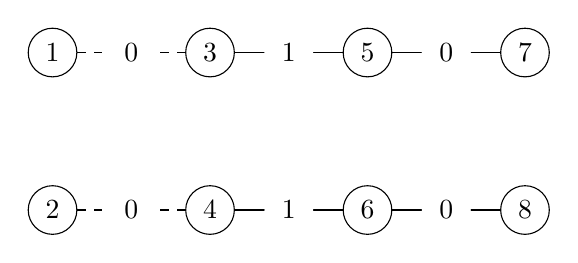
\begin{tikzpicture}

      \begin{scope}[every node/.style={circle,draw}]
        \node (1) at (0,2) {1};
        \node (2) at (0,0) {2};
        \node (3) at (2,2) {3};
        \node (4) at (2,0) {4};
        \node (5) at (4,2) {5};
        \node (6) at (4,0) {6};
        \node (7) at (6,2) {7};
        \node (8) at (6,0) {8};
      \end{scope}

      \begin{scope}[every node/.style={fill=white,circle}]

        \begin{scope}[every edge/.style={draw}]
          \path (3) edge node {$1$} (5);
          \path (4) edge node {$1$} (6);
          \path (5) edge node {$2$} (7);
          \path (6) edge node {$2$} (8);
        \end{scope}

        \begin{scope}[every edge/.style={draw,dashed}]
          \path (1) edge node {$0$} (3);
          \path (2) edge node {$0$} (4);
          \path (5) edge node {$0$} (7);
          \path (6) edge node {$0$} (8);
        \end{scope}

      \end{scope}

    \end{tikzpicture}
  \end{center}

  \begin{center}
    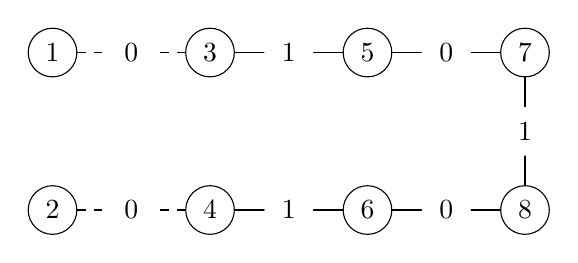
\begin{tikzpicture}

      \begin{scope}[every node/.style={circle,draw}]
        \node (1) at (0,2) {1};
        \node (2) at (0,0) {2};
        \node (3) at (2,2) {3};
        \node (4) at (2,0) {4};
        \node (5) at (4,2) {5};
        \node (6) at (4,0) {6};
        \node (7) at (6,2) {7};
        \node (8) at (6,0) {8};
      \end{scope}

      \begin{scope}[every node/.style={fill=white,circle}]

        \begin{scope}[every edge/.style={draw}]
          \path (3) edge node {$1$} (5);
          \path (4) edge node {$1$} (6);
          \path (5) edge node {$2$} (7);
          \path (6) edge node {$2$} (8);
          \path (7) edge node {$1$} (8);
        \end{scope}

        \begin{scope}[every edge/.style={draw,dashed}]
          \path (1) edge node {$0$} (3);
          \path (2) edge node {$0$} (4);
          \path (5) edge node {$0$} (7);
          \path (6) edge node {$0$} (8);
        \end{scope}

      \end{scope}

    \end{tikzpicture}
  \end{center}



  \begin{center}
    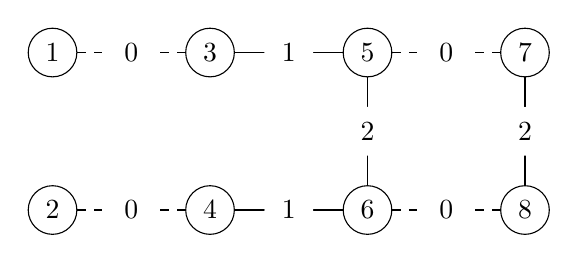
\begin{tikzpicture}

      \begin{scope}[every node/.style={circle,draw}]
        \node (1) at (0,2) {1};
        \node (2) at (0,0) {2};
        \node (3) at (2,2) {3};
        \node (4) at (2,0) {4};
        \node (5) at (4,2) {5};
        \node (6) at (4,0) {6};
        \node (7) at (6,2) {7};
        \node (8) at (6,0) {8};
      \end{scope}

      \begin{scope}[every node/.style={fill=white,circle}]

        \begin{scope}[every edge/.style={draw}]
          \path (3) edge node {$1$} (5);
          \path (4) edge node {$1$} (6);
          \path (5) edge node {$2$} (6);
          \path (7) edge node {$2$} (8);
        \end{scope}

        \begin{scope}[every edge/.style={draw,dashed}]
          \path (1) edge node {$0$} (3);
          \path (2) edge node {$0$} (4);
          \path (5) edge node {$0$} (7);
          \path (6) edge node {$0$} (8);
        \end{scope}

      \end{scope}

    \end{tikzpicture}
  \end{center}

  \begin{center}
    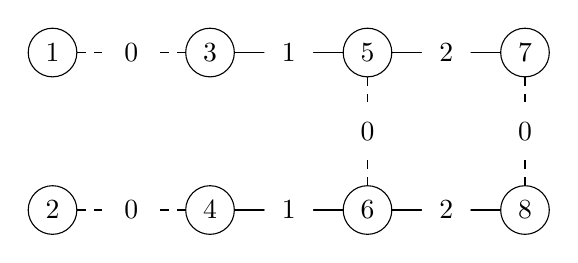
\begin{tikzpicture}

      \begin{scope}[every node/.style={circle,draw}]
        \node (1) at (0,2) {1};
        \node (2) at (0,0) {2};
        \node (3) at (2,2) {3};
        \node (4) at (2,0) {4};
        \node (5) at (4,2) {5};
        \node (6) at (4,0) {6};
        \node (7) at (6,2) {7};
        \node (8) at (6,0) {8};
      \end{scope}

      \begin{scope}[every node/.style={fill=white,circle}]

        \begin{scope}[every edge/.style={draw}]
          \path (3) edge node {$1$} (5);
          \path (4) edge node {$1$} (6);
          \path (5) edge node {$2$} (7);
          \path (6) edge node {$2$} (8);

        \end{scope}

        \begin{scope}[every edge/.style={draw,dashed}]
          \path (1) edge node {$0$} (3);
          \path (2) edge node {$0$} (4);
          \path (5) edge node {$0$} (6);
          \path (7) edge node {$0$} (8);

        \end{scope}

      \end{scope}

    \end{tikzpicture}
  \end{center}

  \paragraph{}
  Essayons de construire un graphe valide à 9 points. Considérons les deux dernier graphes de l'étape précédente, ceux-ci sont presque indentiques. Vu que nous allons tenter d'accrocher un sommet sur 5, 6, 7 ou 8 nous les considérerons comme identiques. Si nous voulons accrocher un sommet tout en restant en rang 3, nous devons utiliser soit 7 soit 8 (mais c'est pareil). Si nous ne l'accrochons qu'une fois l'involution 1 est impaire. Mais si nous l'accrochons 2 fois, le sommet 9 serait permuté deux fois par la même involution. Donc il faut augmenter le rang.

  \paragraph{}
  Si nous agmentons le rang, nous créeons une involution 3. Cette involution devra relier le sommet 9 à un autre. Mais il devra y avoir deux autres sommets permutés par 3 pour que cette involutions soit paire. La seule possibilité est d'inverser 7 et 8. Mais alors, le sommet devrait venir s'accorcher sur 5 ou 6 et ne pourrait pas former un carré avec l'involution 0 (car 3 et 4 sont fixés). Donc il est impossible de trouver un graphe satisfaisant sur 9 sommets.

  \paragraph{}
  Étendons nos constructions à 10 sommets. Encore une fois nous pouvons soit ajouter un sommet par ligne soit deux sommets sur la ligne du dessus, dans ce cas ils ne pouront pas être reliés au sommet 8.

  \paragraph{}
  Regardons ce dernier cas, dans les deux derniers graphes de l'étape précédente, on peut rajouter une arête entre 9 et 7. Il est impossible de se raccorder sur 5 car on ne saurait pas former un carré sur 3 ou 4. Si on se raccorde sur 7, on est obligé d'utiliser l'involution 1. Pour relier le point 10, on est obligé de le relier à 9. En effet si on le reliait à 7, avec une nouvelle involution 3, il ne formerait pas un carré avec l'involution 1. En le reliant à 9, on peut choisir entre l'involution 0 ou 2 ou les deux. On trouve donc les cas suivants.

  \begin{center}
    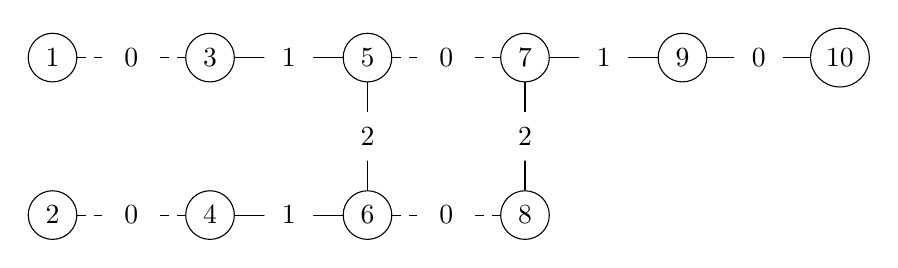
\begin{tikzpicture}

      \begin{scope}[every node/.style={circle,draw}]
        \node (1) at (0,2) {1};
        \node (2) at (0,0) {2};
        \node (3) at (2,2) {3};
        \node (4) at (2,0) {4};
        \node (5) at (4,2) {5};
        \node (6) at (4,0) {6};
        \node (7) at (6,2) {7};
        \node (8) at (6,0) {8};
        \node (9) at (8,2) {9};
        \node (10) at (10,2) {10};
      \end{scope}

      \begin{scope}[every node/.style={fill=white,circle}]

        \begin{scope}[every edge/.style={draw}]
          \path (3) edge node {$1$} (5);
          \path (4) edge node {$1$} (6);
          \path (5) edge node {$2$} (6);
          \path (7) edge node {$2$} (8);
          \path (7) edge node {$1$} (9);
          \path (9) edge node {$2$} (10);
        \end{scope}

        \begin{scope}[every edge/.style={draw,dashed}]
          \path (1) edge node {$0$} (3);
          \path (2) edge node {$0$} (4);
          \path (5) edge node {$0$} (7);
          \path (6) edge node {$0$} (8);
          \path (9) edge node {$0$} (10);
        \end{scope}

      \end{scope}

    \end{tikzpicture}
  \end{center}

  \begin{center}
    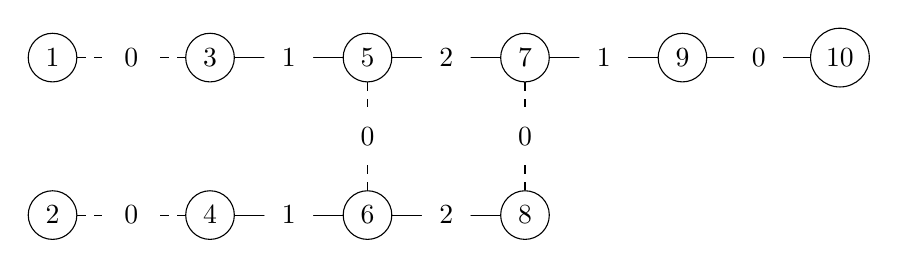
\begin{tikzpicture}

      \begin{scope}[every node/.style={circle,draw}]
        \node (1) at (0,2) {1};
        \node (2) at (0,0) {2};
        \node (3) at (2,2) {3};
        \node (4) at (2,0) {4};
        \node (5) at (4,2) {5};
        \node (6) at (4,0) {6};
        \node (7) at (6,2) {7};
        \node (8) at (6,0) {8};
        \node (9) at (8,2) {9};
        \node (10) at (10,2) {10};
      \end{scope}

      \begin{scope}[every node/.style={fill=white,circle}]

        \begin{scope}[every edge/.style={draw}]
          \path (3) edge node {$1$} (5);
          \path (4) edge node {$1$} (6);
          \path (5) edge node {$2$} (7);
          \path (6) edge node {$2$} (8);
          \path (7) edge node {$1$} (9);
          \path (9) edge node {$2$} (10);
        \end{scope}

        \begin{scope}[every edge/.style={draw,dashed}]
          \path (1) edge node {$0$} (3);
          \path (2) edge node {$0$} (4);
          \path (5) edge node {$0$} (6);
          \path (7) edge node {$0$} (8);
          \path (9) edge node {$0$} (10);
        \end{scope}

      \end{scope}

    \end{tikzpicture}
  \end{center}

  \paragraph{}
  Pour le deuxième graphe, si 5--7 est l'involution 0, alors 7--9 doit être l'involution 2. Mais il faudrait former un cycle avec 5 ce qui est possible si 9--10 est 0 et 10--5 est 2. Le cas d'une nouvelle involution 3 est impossible car sinon elle devrait former un carré avec 1.

  \paragraph{}
  Si 5--7 est l'involution 2 alors 7--9 doit être 0 et former un carré via 9--10 qui est 2 et 10--7 qui est 0. Encore une fois le cas d'une nouvelle involution est exclu. On a donc les possibilités suivantes:

  \begin{center}
    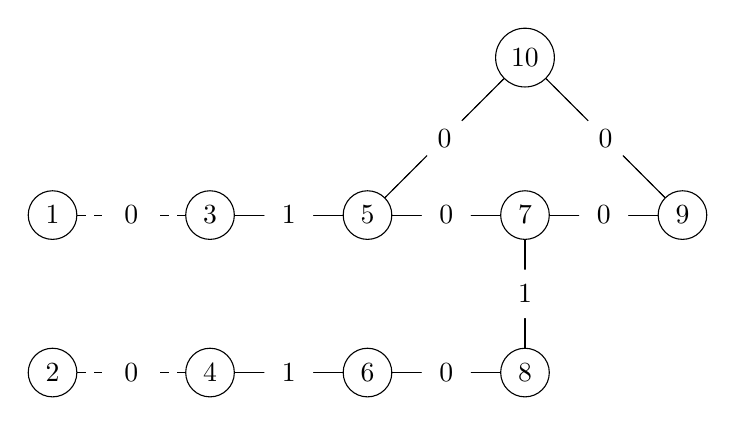
\begin{tikzpicture}

      \begin{scope}[every node/.style={circle,draw}]
        \node (1) at (0,2) {1};
        \node (2) at (0,0) {2};
        \node (3) at (2,2) {3};
        \node (4) at (2,0) {4};
        \node (5) at (4,2) {5};
        \node (6) at (4,0) {6};
        \node (7) at (6,2) {7};
        \node (8) at (6,0) {8};
        \node (9) at (8,2) {9};
        \node (10) at (6,4) {10};
      \end{scope}

      \begin{scope}[every node/.style={fill=white,circle}]

        \begin{scope}[every edge/.style={draw}]
          \path (3) edge node {$1$} (5);
          \path (4) edge node {$1$} (6);
          \path (5) edge node {$2$} (7);
          \path (6) edge node {$2$} (8);
          \path (7) edge node {$1$} (8);
          \path (7) edge node {$2$} (9);
          \path (9) edge node {$2$} (10);
          \path (10) edge node {$2$} (5);
        \end{scope}

        \begin{scope}[every edge/.style={draw,dashed}]
          \path (1) edge node {$0$} (3);
          \path (2) edge node {$0$} (4);
          \path (5) edge node {$0$} (7);
          \path (6) edge node {$0$} (8);
          \path (7) edge node {$0$} (9);
          \path (9) edge node {$0$} (10);
          \path (10) edge node {$0$} (5);
        \end{scope}

      \end{scope}

    \end{tikzpicture}
  \end{center}

  \paragraph{}
  Si nous partons du premier graphe. Si 5--7 contient l'involution 0, alors 7--9 doit être l'involution 1. Dans le cas contraire 1 et 3 sont des solutions envisageables. Pour relier 10, nous devons utiliser 0, 2 ou 4. On ne peut pas relier au 6 car on devrait former un carré et donc relier le 8 aussi. On a donc les graphes suivants:

  \begin{center}
    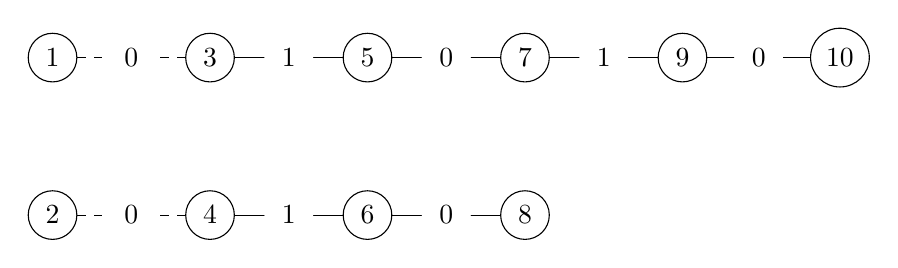
\begin{tikzpicture}

      \begin{scope}[every node/.style={circle,draw}]
        \node (1) at (0,2) {1};
        \node (2) at (0,0) {2};
        \node (3) at (2,2) {3};
        \node (4) at (2,0) {4};
        \node (5) at (4,2) {5};
        \node (6) at (4,0) {6};
        \node (7) at (6,2) {7};
        \node (8) at (6,0) {8};
        \node (9) at (8,2) {9};
        \node (10) at (10,2) {10};
      \end{scope}

      \begin{scope}[every node/.style={fill=white,circle}]

        \begin{scope}[every edge/.style={draw}]
          \path (3) edge node {$1$} (5);
          \path (4) edge node {$1$} (6);
          \path (5) edge node {$2$} (7);
          \path (6) edge node {$2$} (8);
          \path (7) edge node {$1$} (9);
          \path (9) edge node {$2$} (10);
        \end{scope}

        \begin{scope}[every edge/.style={draw,dashed}]
          \path (1) edge node {$0$} (3);
          \path (2) edge node {$0$} (4);
          \path (5) edge node {$0$} (7);
          \path (6) edge node {$0$} (8);
          \path (9) edge node {$0$} (10);
        \end{scope}

      \end{scope}

    \end{tikzpicture}
  \end{center}

  \begin{center}
    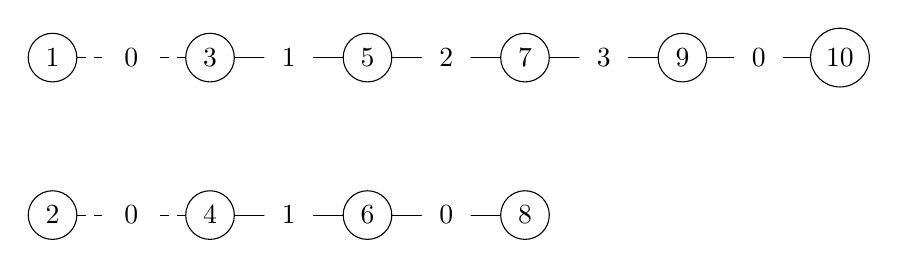
\begin{tikzpicture}

      \begin{scope}[every node/.style={circle,draw}]
        \node (1) at (0,2) {1};
        \node (2) at (0,0) {2};
        \node (3) at (2,2) {3};
        \node (4) at (2,0) {4};
        \node (5) at (4,2) {5};
        \node (6) at (4,0) {6};
        \node (7) at (6,2) {7};
        \node (8) at (6,0) {8};
        \node (9) at (8,2) {9};
        \node (10) at (10,2) {10};
      \end{scope}

      \begin{scope}[every node/.style={fill=white,circle}]

        \begin{scope}[every edge/.style={draw}]
          \path (3) edge node {$1$} (5);
          \path (4) edge node {$1$} (6);
          \path (5) edge node {$2$} (7);
          \path (6) edge node {$2$} (8);
          \path (7) edge node {$1$} (9);
          \path (7) edge node {$3$} (9);
          \path (9) edge node {$2$} (10);
        \end{scope}

        \begin{scope}[every edge/.style={draw,dashed}]
          \path (1) edge node {$0$} (3);
          \path (2) edge node {$0$} (4);
          \path (6) edge node {$0$} (8);
          \path (9) edge node {$0$} (10);
        \end{scope}

      \end{scope}

    \end{tikzpicture}
  \end{center}

  \paragraph{}
  Si on en rajoute un sur chaque ligne et si on considère les deux derniers graphes du cas précédent, on trouve que 9 doit être relié à 5 ou 7 (par symmétrie) mais 5 est impossible car on ne forme pas de carré avec l'involution 1. Donc il doit être relié à 7.

  \paragraph{}
  Dans le troisième graphe, on est obligé d'utiliser l'involution 1 car sinon on ne forme pas de carré avec 0. Dans le quatrième cas, on peut utiliser soit l'involution 1, soit une nouvelle involution 3 et créer un lien entre 9 et 10 avec l'involution 0 pour former un carré. On a donc les 3 cas suivants:

  \begin{center}
    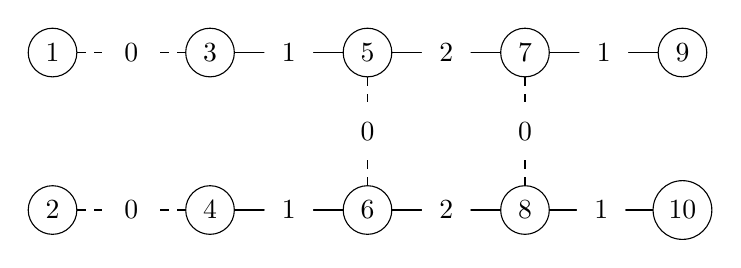
\begin{tikzpicture}

      \begin{scope}[every node/.style={circle,draw}]
        \node (1) at (0,2) {1};
        \node (2) at (0,0) {2};
        \node (3) at (2,2) {3};
        \node (4) at (2,0) {4};
        \node (5) at (4,2) {5};
        \node (6) at (4,0) {6};
        \node (7) at (6,2) {7};
        \node (8) at (6,0) {8};
        \node (9) at (8,2) {9};
        \node (10) at (8,0) {10};
      \end{scope}

      \begin{scope}[every node/.style={fill=white,circle}]

        \begin{scope}[every edge/.style={draw}]
          \path (3) edge node {$1$} (5);
          \path (4) edge node {$1$} (6);
          \path (5) edge node {$2$} (7);
          \path (6) edge node {$2$} (8);
          \path (7) edge node {$1$} (9);
          \path (8) edge node {$1$} (10);
        \end{scope}

        \begin{scope}[every edge/.style={draw,dashed}]
          \path (1) edge node {$0$} (3);
          \path (2) edge node {$0$} (4);
          \path (5) edge node {$0$} (6);
          \path (7) edge node {$0$} (8);
        \end{scope}

      \end{scope}

    \end{tikzpicture}
  \end{center}

  \begin{center}
    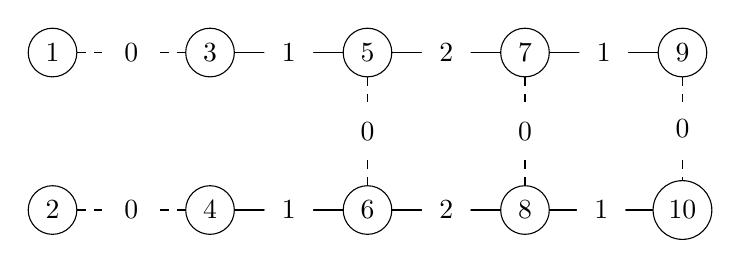
\begin{tikzpicture}

      \begin{scope}[every node/.style={circle,draw}]
        \node (1) at (0,2) {1};
        \node (2) at (0,0) {2};
        \node (3) at (2,2) {3};
        \node (4) at (2,0) {4};
        \node (5) at (4,2) {5};
        \node (6) at (4,0) {6};
        \node (7) at (6,2) {7};
        \node (8) at (6,0) {8};
        \node (9) at (8,2) {9};
        \node (10) at (8,0) {10};
      \end{scope}

      \begin{scope}[every node/.style={fill=white,circle}]

        \begin{scope}[every edge/.style={draw}]
          \path (3) edge node {$1$} (5);
          \path (4) edge node {$1$} (6);
          \path (5) edge node {$2$} (7);
          \path (6) edge node {$2$} (8);
          \path (7) edge node {$1$} (9);
          \path (8) edge node {$1$} (10);
        \end{scope}

        \begin{scope}[every edge/.style={draw,dashed}]
          \path (1) edge node {$0$} (3);
          \path (2) edge node {$0$} (4);
          \path (5) edge node {$0$} (6);
          \path (7) edge node {$0$} (8);
          \path (9) edge node {$0$} (10);
        \end{scope}

      \end{scope}

    \end{tikzpicture}
  \end{center}

  \begin{center}
    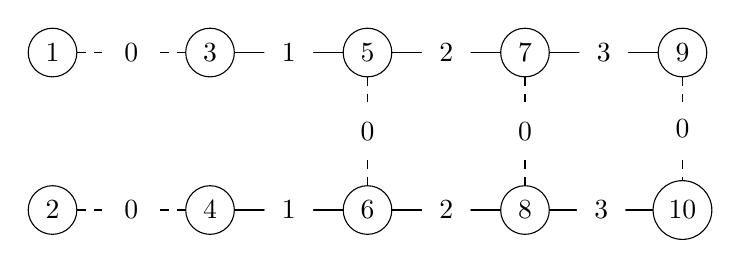
\begin{tikzpicture}

      \begin{scope}[every node/.style={circle,draw}]
        \node (1) at (0,2) {1};
        \node (2) at (0,0) {2};
        \node (3) at (2,2) {3};
        \node (4) at (2,0) {4};
        \node (5) at (4,2) {5};
        \node (6) at (4,0) {6};
        \node (7) at (6,2) {7};
        \node (8) at (6,0) {8};
        \node (9) at (8,2) {9};
        \node (10) at (8,0) {10};
      \end{scope}

      \begin{scope}[every node/.style={fill=white,circle}]

        \begin{scope}[every edge/.style={draw}]
          \path (3) edge node {$1$} (5);
          \path (4) edge node {$1$} (6);
          \path (5) edge node {$2$} (7);
          \path (6) edge node {$2$} (8);
          \path (7) edge node {$3$} (9);
          \path (8) edge node {$3$} (10);
        \end{scope}

        \begin{scope}[every edge/.style={draw,dashed}]
          \path (1) edge node {$0$} (3);
          \path (2) edge node {$0$} (4);
          \path (5) edge node {$0$} (6);
          \path (7) edge node {$0$} (8);
          \path (9) edge node {$0$} (10);
        \end{scope}

      \end{scope}

    \end{tikzpicture}
  \end{center}

  \paragraph{}
  Pour le deuxième cas, si l'arête 5--7 est un 0, on ne peut pas relier 7 et 9 par une arête car on doit utiliser l'involution 2 ou une nouvelle involution 3 mais dans les deux cas, on ne sait pas former un carré avec l'involution 0. Le problème est le même si on tante de le relier au 5.

  \paragraph{}
  Donc l'arête 5--7 et donc 6-8 doivent être l'involution 2. Dans ce cas, on peut utiliser l'involution 0 ou une nouvelle involution 3. Si on utilise 0, on se sait pas former un carré avec l'involution 2 de 5--7. Donc on doit utiliser l'involution 3. Mais il faut qu'elle forme un carré avec l'involution 1. Ce qui n'est possible que si 9 et 10 sont relié par l'involution 1. On n'a donc qu'une seule possibilité dans ce cas qui est

  \begin{center}
    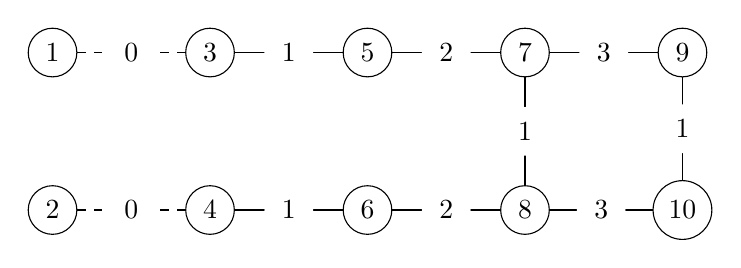
\begin{tikzpicture}

      \begin{scope}[every node/.style={circle,draw}]
        \node (1) at (0,2) {1};
        \node (2) at (0,0) {2};
        \node (3) at (2,2) {3};
        \node (4) at (2,0) {4};
        \node (5) at (4,2) {5};
        \node (6) at (4,0) {6};
        \node (7) at (6,2) {7};
        \node (8) at (6,0) {8};
        \node (9) at (8,2) {9};
        \node (10) at (8,0) {10};
      \end{scope}

      \begin{scope}[every node/.style={fill=white,circle}]

        \begin{scope}[every edge/.style={draw}]
          \path (3) edge node {$1$} (5);
          \path (4) edge node {$1$} (6);
          \path (5) edge node {$2$} (7);
          \path (6) edge node {$2$} (8);
          \path (7) edge node {$1$} (8);
          \path (7) edge node {$3$} (9);
          \path (8) edge node {$3$} (10);
          \path (9) edge node {$1$} (10);
        \end{scope}

        \begin{scope}[every edge/.style={draw,dashed}]
          \path (1) edge node {$0$} (3);
          \path (2) edge node {$0$} (4);
        \end{scope}

      \end{scope}

    \end{tikzpicture}
  \end{center}

  \paragraph{}
  Regardons maintenant le premier graphe, si l'arête 5--7 est 0 ou double alors, l'arête 7--9 doit être l'involution 1. Si 5--7 est 2, alors 7--9 peut être 1 ou 3 ou un arête double. Le même raisonnemeent tient pour 8--10.

  \paragraph{}
  Nous pouvons toujours attacher 9 et 10 avec, au choix un arête 0, 2 ou 4 ou une combinaison de celles-ci.


  \paragraph{}
  Essayons maintenant de construire un graphe valide à 11 points. Si deux points sont rajoutés sur la ligne du haut.

  \paragraph{}
  Dans les deux premiers graphes, l'involution 0 ou 2 est de degré impair mais nous n'avons aucun point d'attache.

  \paragraph{}
  Le même raisonnement tient dans le troisième graphe.

  \paragraph{}
  Pour les troisième graphe, le nombre de 1 est impair. On a pas de point d'accroche.

  \paragraph{}
  Dans le dernier graphe, si le 3 n'est pas présent on a trois involutions 1. Le seul point d'accroche est le 8. Il faut que le graphe soit transitif donc il faut l'accorcher à la ligne du haut aussi. On doit utiliser un 0 ou un 2 car les autres sont toujours pairs. Mais on ne sait pas l'accrocher.

  \paragraph{}
  Si le 3 est présent, alors on doit relier le point 11 avec un 3. Soit au point 8 si 6--8 ne contient pas de 2, soit au point 10. Dans le premier cas, il faut encore relier 11 à la première ligne avec soit un 2 soit un 4, mais c'est impossible. Si on accroche au 10, on arrive au même résultat.


  \paragraph{}
  Regardons maintenant les cas où un point est rajouté sur chaque ligne.

  \paragraph{}
  Dans les deux premiers cas, nous avons un nombre impair d'involution 1 donc nous sommes obligés de raccorder notre point 11 par une involution 1 au point 8 car c'est le seul point qui n'est pas fixé ou déjà relié par une involution 1. Mais nous avons aussi une involution 0 et/ou 2 qui est impair et il est impossible de raccorder le point 11 à un sommet car ils sont tous fixés ou déjà raccordé.

  \paragraph{}
  Pour le troisième cas, regardons nos 3 graphes, dans le deux derniers on a un nombre impair d'involutions 0, donc notre point 11 doit être relié par une involution 0 mais il n'y a aucun point d'attache disponible.

  \paragraph{}
  Dans le premier graphe, nous ne pouvons pas utiliser une nouvelle involution car sinon elle serait impaire. De même, vu que toutes les involutions existantes sont paires, il est impossible d'utiliser une involution existante.

  \paragraph{}
  Dans le cas suivant, toutes les involutions sont déjà paires donc c'est impossible.

  \paragraph{}
  Dans le dernier cas, nous devons avoir un nombre impair d'au moins une involution. Si cette involution est 0, elle ne doit apparaître qu'une fois, sinon nous n'avons pas de point d'accroche. Mais ce point d'accroche va forcément déjà lier un 2 ou un 4. Et vu qu'il s'agit d'un chemin, il n'est pas possible de créer un carré en ajoutant un sommet. Idem pour 2 et 4.

  \paragraph{}
  À partir de 13 points, on trouve des contre-exemples:

  \begin{center}
    \begin{tikzpicture}

      \begin{scope}[every node/.style={circle,draw}]
        \node (1)  at (0,2)  {1};
        \node (2)  at (0,0)  {2};
        \node (3)  at (2,2)  {3};
        \node (4)  at (2,0)  {4};
        \node (5)  at (4,2)  {5};
        \node (6)  at (4,0)  {6};
        \node (7)  at (6,2)  {7};
        \node (8)  at (6,0)  {8};
        \node (9)  at (8,2)  {9};
        \node (10) at (8,0)  {10};
        \node (11) at (10,2) {11};
        \node (13) at (6,4)  {12};
        \node (14) at (6,-2) {13};
      \end{scope}

      \begin{scope}[every node/.style={fill=white,circle}]

        \begin{scope}[every edge/.style={draw}]
          \path (3)  edge node {$1$} (5);
          \path (4)  edge node {$1$} (6);
          \path (7)  edge node {$1$} (8);
          \path (7)  edge node {$2$} (9);
          \path (8)  edge node {$2$} (10);
          \path (9)  edge node {$1$} (11);
          \path (5)  edge node {$2$} (13);
          \path (6)  edge node {$2$} (14);
        \end{scope}

        \begin{scope}[every edge/.style={draw,dashed}]
          \path (1)  edge node {$0$} (3);
          \path (2)  edge node {$0$} (4);
          \path (5)  edge node {$0$} (7);
          \path (6)  edge node {$0$} (8);
          \path (10) edge node {$0$} (14);
          \path (9)  edge node {$0$} (13);
        \end{scope}

      \end{scope}

    \end{tikzpicture}
  \end{center}

  \begin{center}
    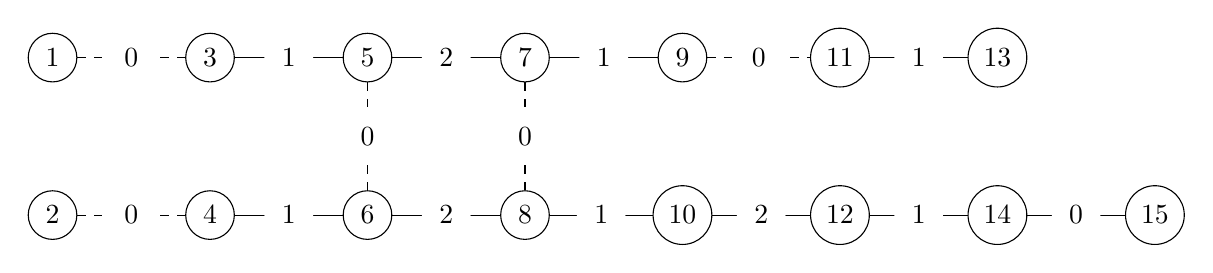
\begin{tikzpicture}

      \begin{scope}[every node/.style={circle,draw}]
        \node (1)  at (0,2)  {1};
        \node (2)  at (0,0)  {2};
        \node (3)  at (2,2)  {3};
        \node (4)  at (2,0)  {4};
        \node (5)  at (4,2)  {5};
        \node (6)  at (4,0)  {6};
        \node (7)  at (6,2)  {7};
        \node (8)  at (6,0)  {8};
        \node (9)  at (8,2)  {9};
        \node (10) at (8,0)  {10};
        \node (11) at (10,2) {11};
        \node (12) at (10,0) {12};
        \node (13) at (12,2)  {13};
        \node (14) at (12,0)  {14};
        \node (15) at (14,0) {15};
      \end{scope}

      \begin{scope}[every node/.style={fill=white,circle}]

        \begin{scope}[every edge/.style={draw}]
          \path (3)  edge node {$1$} (5);
          \path (4)  edge node {$1$} (6);
          \path (5)  edge node {$2$} (7);
          \path (6)  edge node {$2$} (8);
          \path (7)  edge node {$1$} (9);
          \path (8)  edge node {$1$} (10);
          \path (10) edge node {$2$} (12);
          \path (11) edge node {$1$} (13);
          \path (12) edge node {$1$} (14);
          \path (14) edge node {$2$} (15);
        \end{scope}

        \begin{scope}[every edge/.style={draw,dashed}]
          \path (1)  edge node {$0$} (3);
          \path (2)  edge node {$0$} (4);
          \path (5)  edge node {$0$} (6);
          \path (7)  edge node {$0$} (8);
          \path (9)  edge node {$0$} (11);
          \path (14) edge node {$0$} (15);
        \end{scope}

      \end{scope}

    \end{tikzpicture}
  \end{center}

\end{proof}

\cleardoublepage{}

\section{Réécriture}

\subsection{Introduction}

\begin{theorem}
  Soit $G$ un groupe transitif et soit $H$ un sous-groupe qui fixe deux points et qui est un string C-group généré par les involutions $\rho_1, \dots, \rho_n$. Alors il est impossible d'étendre à $G$ ce string C-group avec les involutions $\rho_0, \dots, \rho_n$ si $G$ est composé uniquement de permutations impaires et
  \begin{itemize}
    \item si le degré de $G$ est pair et est strictement inférieur à 8 ou
    \item si le degré de $G$ est impaire et est strictement inférieur à 13.
  \end{itemize}
\end{theorem}

\paragraph{}
Pour prouver ce théorème, nous allons construire tous les multigraphes correspondants à des sggi. Si nous n'arrivons à en construire aucun, celà signifie qu'il n'existe pas de string C-group de ce degré.

\paragraph{}
Lorsque nous ajoutons un point, nous pouvons faire le relier par une ou plusieurs involution(s) existante(s) ou nouvelle(s) à un ou plusieurs point(s) existants.
Néanmoins, il n'est pas envisageable d'ajouter une involution entre deux points dejà existants, que l'involution soit nouvelle ou pas. En effet, ce lien a déjà été envisagé lorsque nous avons placé nos points.

\paragraph{}
Néanmoins, nous allons toujours ajouter les points par deux. Vu que pour que le multigraphe soit un graphe de sggi valable, il faut que des arêtes avec des indices non consécutifs forment des points, des lignes simples, des lignes doubles ou des carrés. Dans ce dernier cas, il est nécessaire d'ajouter deux points pour pouvoir les former, d'où notre choix.

\paragraph{}
Les deux points fixes de $H$ seront nommés, par convention, 1 et 2. De même l'involution ajoutée sera nommée $\rho_0$.

\paragraph{}
Rappelons les contraintes, 1 et 2 sont des points fixes de $H$, ce qui implique que
\begin{center}
  $1 \rho_i = 1$ et $2 \rho_i = 2$ si $i \neq 0$.
\end{center}
Le graphe, pour être valide doit uniquement être composé d'involutions paires et est connexe en plus de satisfaire aux conditions d'un graphe de sggi.

\paragraph{}
Cependant, pour pouvoir vérifier si on peut construire les graphes pour les degrés impairs, nous serons amener à ajouter un unique point. Même si ces constructions ne seront pas étendues, il est intéressant de noter les quelques propriétés ci-dessous afin de pouvoir éliminer certains cas d'avance.

\begin{lemma}\label{attachEven}
  Il est impossible d'attacher un sommet unique sur un graphe dont toutes les involutions sont paires.
\end{lemma}

\begin{lemma}\label{attachConnexEven}
  Il est impossible d'attacher un sommet unique sur un graphe non connexe qui ne possède pas au moins deux involutions impaires.
\end{lemma}

\begin{lemma}\label{attachNoFixedPoint}
  Il est impossible d'attacher un sommet unique sur un graphe pour lequel une involution impaire n'a aucun point fixe.
\end{lemma}

\subsection{Degré 2}

\paragraph{}
Si nous n'avons que deux points, $H$ est en fait vide et ne contient aucune involution.

\paragraph{}
Nous avons donc deux possibilités, soit nous relions les deux points entre eux avec l'involution 0 (vu que les autres sont interdites), soit nous ne le faisons pas. Cela nous donne les deux graphes \ref{f.d2.l} et \ref{f.d2.nl}.


\begin{figure}[H]
  \begin{center}
    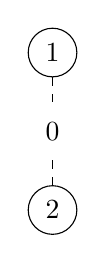
\begin{tikzpicture}

      \begin{scope}[every node/.style={circle,draw}]
        \node (1)  at (0,2)  {1};
        \node (2)  at (0,0)  {2};
      \end{scope}

      \begin{scope}[every node/.style={fill=white,circle}]

        \begin{scope}[every edge/.style={draw}]

        \end{scope}

        \begin{scope}[every edge/.style={draw,dashed}]
          \path (1)  edge node {$0$} (2);
        \end{scope}

      \end{scope}

    \end{tikzpicture}
  \end{center}
  \caption{Degré deux, reliés}
  \label{f.d2.l}
\end{figure}

\begin{figure}[H]
  \begin{center}
    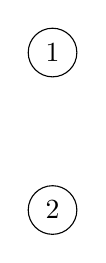
\begin{tikzpicture}

      \begin{scope}[every node/.style={circle,draw}]
        \node (1)  at (0,2)  {1};
        \node (2)  at (0,0)  {2};
      \end{scope}

      \begin{scope}[every node/.style={fill=white,circle}]

        \begin{scope}[every edge/.style={draw}]

        \end{scope}

        \begin{scope}[every edge/.style={draw,dashed}]

        \end{scope}

      \end{scope}

    \end{tikzpicture}
  \end{center}
  \caption{Degré deux, non reliés}
  \label{f.d2.nl}
\end{figure}

\paragraph{}
Vérifions si ces graphes sont des graphes satisfaisant aux conditions. Dans le graphe \ref{f.d2.l}, l'involution $\rho_0$ est impaire donc ce n'est pas valide. Pour le cas \ref{f.d2.nl}, le graphe n'est pas connexe.

\subsection{Degré 3}

\paragraph{}
On ne sait pas attacher de point a graphe \ref{f.d2.l} par le lemme \ref{attachNoFixedPoint}. De même pour le graphe \ref{f.d2.nl}, par le lemme \ref{attachEven}.

\subsection{Degré 4}

\paragraph{}
Nous allons tenter d'étendre les graphes de degré 2 à des graphes de degré 4.

\paragraph{}
En partant du graphe \ref{f.d2.l}, nous ne pouvons pas trouver de graphe plus grand transitif. En effet les points 1 et 2 dont des points fixes pour toutes les involutions sauf $\rho_0$. Donc l'orbite de ces deux points sera toujours $\{1, 2\}$ et donc le graphe ne sera jamais connexe.

\paragraph{}
En partant du graphe \ref{f.d2.nl}, nous devons ajouter deux points : 3 et 4. Il faut que 3 soit connecté à 1. En effet, nous avons convenu que les points que nous ajoutons doivent être connecté à au moins un point du graphe existant. Pour éviter les doublons, nous imposons que ça soit 1. Si ça devait être 2, il suffit de renommer 3 en 4 et inversément.

\paragraph{}
Pour relier 1 et 3, nous sommes obligés d'utilise l'involution $\rho_0$, car c'est la seule acceptable pour le sommet 1.

\paragraph{}
Pour le point 4, nous avons deux possibilités, soit nous le relions à 2, soit nous le relions à 3 sans le relier à 2. Cependant vu que le graphe partiel que nous avons n'est pas transitif, le point 2 devra être relié à un autre sommet plus tard et donc nous pouvons considérer que nous sommes obligés de relier 2 et 4, toujours avec l'involution $\rho_0$.

\paragraph{}
Il nous reste encore à décider si les deux points que nous avons ajouté seront reliés ou pas. Rien ne s'y oppose, pour autant que nous utilisions une nouvelle involution $\rho_1$ (le cas avec une autre involution est impossible voir plus bas). Nous pouvons donc envisager le deux cas.

\paragraph{}
Les graphes que nous avons à ce momement sont les graphes \ref{f.d4.l} et \ref{f.d4.nl}.

\begin{figure}[H]
  \begin{center}
    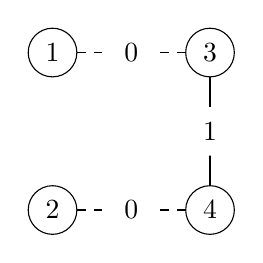
\begin{tikzpicture}

      \begin{scope}[every node/.style={circle,draw}]
        \node (1)  at (0,2)  {1};
        \node (2)  at (0,0)  {2};
        \node (3)  at (2,2)  {3};
        \node (4)  at (2,0)  {4};
      \end{scope}

      \begin{scope}[every node/.style={fill=white,circle}]

        \begin{scope}[every edge/.style={draw}]
          \path (3)  edge node {$1$} (4);
        \end{scope}

        \begin{scope}[every edge/.style={draw,dashed}]
          \path (1)  edge node {$0$} (3);
          \path (2)  edge node {$0$} (4);
        \end{scope}

      \end{scope}

    \end{tikzpicture}
  \end{center}
  \caption{Degré quatre, reliés}
  \label{f.d4.l}
\end{figure}


\begin{figure}[H]
  \begin{center}
    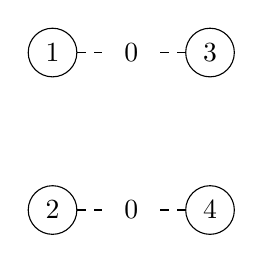
\begin{tikzpicture}

      \begin{scope}[every node/.style={circle,draw}]
        \node (1)  at (0,2)  {1};
        \node (2)  at (0,0)  {2};
        \node (3)  at (2,2)  {3};
        \node (4)  at (2,0)  {4};
      \end{scope}

      \begin{scope}[every node/.style={fill=white,circle}]

        \begin{scope}[every edge/.style={draw}]

        \end{scope}

        \begin{scope}[every edge/.style={draw,dashed}]
          \path (1)  edge node {$0$} (3);
          \path (2)  edge node {$0$} (4);
        \end{scope}

      \end{scope}

    \end{tikzpicture}
  \end{center}
  \caption{Degré quater, non reliés}
  \label{f.d4.nl}
\end{figure}

\subsection{Degré 5}

\paragraph{}
Pour le graphe, \ref{f.d4.l} on peut utiliser le lemme \ref{attachNoFixedPoint}, vu que 1 et 2 sont des points fixes pour toutes les involutions sauf $\rho_0$.

\paragraph{}
Pour le graphe \ref{f.d4.nl}, on peut conclure avec le lemme \ref{attachEven}.

\subsection{Degré 6}

\paragraph{}
Commençons par remarquer que les points 3 et 4 sont des points fixes pour les involution $\rho_i$ avec $i \ge 2$. En effet si 3 n'était pas un point fixe pour $\rho_2$. Il faudrait qu'il existe un carré alterné avec les involutions $\rho_0$ et $\rho_2$ mais c'est impossible car 1 est un point fixe pour $\rho_2$.

\paragraph{}
À partir de la constatation précédente, il est impossible d'étendre le graphe \ref{f.d4.l}.

\paragraph{}
Concernant le grahe \ref{f.d4.nl}, on doit ajouter un point sur chaque ligne (les arguments sont les mêmes qu'à l'étape précédente). Le point 5 doit être relié au point 3. Vu la remarque ci-dessus, l'involution qui les permutent doit être $\rho_1$. Le même raisonnment tient pour 6 et 4.

\paragraph{}
Ensuite les points 5 et 6 peuvent être reliés par certaines involutions. Les seules possibles sont $\rho_0$ et $\rho_2$. En effet, si on utilisait une autre involution, il faudrait former un carré alterné qui viendrait se reconnecter sur le point 3, ce qui contredit notre remarque. Envisageons donc ces cas.

\paragraph{}
On obtient les 4 graphes suivants: \ref{f.d6.l0}, \ref{f.d6.l2}, \ref{f.d6.l02} et \ref{f.d6.nl}.

\begin{figure}[H]
  \begin{center}
    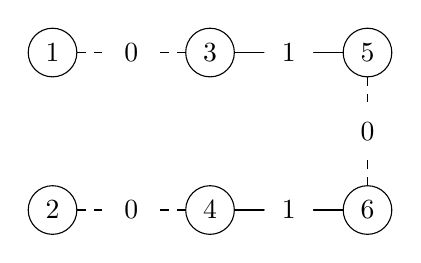
\begin{tikzpicture}

      \begin{scope}[every node/.style={circle,draw}]
        \node (1)  at (0,2)  {1};
        \node (2)  at (0,0)  {2};
        \node (3)  at (2,2)  {3};
        \node (4)  at (2,0)  {4};
        \node (5)  at (4,2)  {5};
        \node (6)  at (4,0)  {6};
      \end{scope}

      \begin{scope}[every node/.style={fill=white,circle}]

        \begin{scope}[every edge/.style={draw}]
          \path (3)  edge node {$1$} (5);
          \path (4)  edge node {$1$} (6);
        \end{scope}

        \begin{scope}[every edge/.style={draw,dashed}]
          \path (1)  edge node {$0$} (3);
          \path (2)  edge node {$0$} (4);
          \path (5)  edge node {$0$} (6);
        \end{scope}

      \end{scope}

    \end{tikzpicture}
  \end{center}
  \caption{Degré six, reliés par $\rho_0$}
  \label{f.d6.l0}
\end{figure}

\begin{figure}[H]
  \begin{center}
    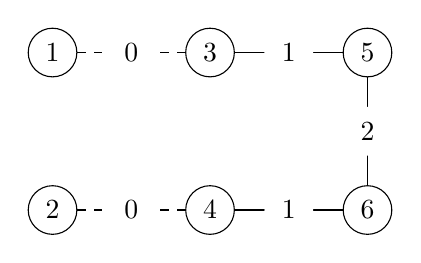
\begin{tikzpicture}

      \begin{scope}[every node/.style={circle,draw}]
        \node (1)  at (0,2)  {1};
        \node (2)  at (0,0)  {2};
        \node (3)  at (2,2)  {3};
        \node (4)  at (2,0)  {4};
        \node (5)  at (4,2)  {5};
        \node (6)  at (4,0)  {6};
      \end{scope}

      \begin{scope}[every node/.style={fill=white,circle}]

        \begin{scope}[every edge/.style={draw}]
          \path (3)  edge node {$1$} (5);
          \path (4)  edge node {$1$} (6);
          \path (5)  edge node {$2$} (6);
        \end{scope}

        \begin{scope}[every edge/.style={draw,dashed}]
          \path (2)  edge node {$0$} (4);
          \path (1)  edge node {$0$} (3);
        \end{scope}

      \end{scope}

    \end{tikzpicture}
  \end{center}
  \caption{Degré six, reliés par $\rho_2$}
  \label{f.d6.l2}
\end{figure}

\begin{figure}[H]
  \begin{center}
    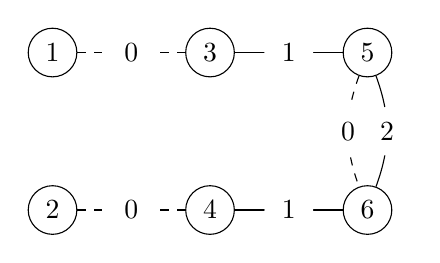
\begin{tikzpicture}

      \begin{scope}[every node/.style={circle,draw}]
        \node (1)  at (0,2)  {1};
        \node (2)  at (0,0)  {2};
        \node (3)  at (2,2)  {3};
        \node (4)  at (2,0)  {4};
        \node (5)  at (4,2)  {5};
        \node (6)  at (4,0)  {6};
      \end{scope}

      \begin{scope}[every node/.style={fill=white,circle}]

        \begin{scope}[every edge/.style={draw}]
          \path (3)  edge node {$1$} (5);
          \path (4)  edge node {$1$} (6);
          \path (5)  edge[bend left=20] node {$2$} (6);
        \end{scope}

        \begin{scope}[every edge/.style={draw,dashed}]
          \path (1)  edge node {$0$} (3);
          \path (2)  edge node {$0$} (4);
          \path (5)  edge[bend right=20] node {$0$} (6);
        \end{scope}

      \end{scope}

    \end{tikzpicture}
  \end{center}
  \caption{Degré six, reliés par $\rho_0$ et $\rho_2$}
  \label{f.d6.l02}
\end{figure}

\begin{figure}[H][H]
  \begin{center}
    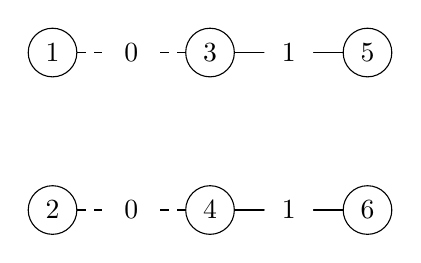
\begin{tikzpicture}

      \begin{scope}[every node/.style={circle,draw}]
        \node (1)  at (0,2)  {1};
        \node (2)  at (0,0)  {2};
        \node (3)  at (2,2)  {3};
        \node (4)  at (2,0)  {4};
        \node (5)  at (4,2)  {5};
        \node (6)  at (4,0)  {6};
      \end{scope}

      \begin{scope}[every node/.style={fill=white,circle}]

        \begin{scope}[every edge/.style={draw}]
          \path (3)  edge node {$1$} (5);
          \path (4)  edge node {$1$} (6);
        \end{scope}

        \begin{scope}[every edge/.style={draw,dashed}]
          \path (1)  edge node {$0$} (3);
          \path (2)  edge node {$0$} (4);
        \end{scope}

      \end{scope}

    \end{tikzpicture}
  \end{center}
  \caption{Degré six, non reliés}
  \label{f.d6.nl}
\end{figure}

Aucun de ces graphes n'est un de ceux que nous recherchons car soit une involution est de degré impair, soit le graphe n'est pas transitif.

\subsection{Degré 7}

\paragraph{}
Pour le graphe \ref{f.d6.l0}, on une impossibilité sur $\rho_0$ par le lemme \ref{attachEven}.

\paragraph{}
Idem pour le graphe \ref{f.d6.l2}, vu que 1, 2, 3 et 4 sont des point fixes pour $\rho_0$.

\paragraph{}
Pour le graphe \ref{f.d6.l02}, les deux arguments précédents tiennent.

\paragraph{}
Pour le graphe \ref{f.d6.nl}, on a une impossibilité par le lemme \ref{attachEven}.

\subsection{Degré 8}

\paragraph{}
Essayons d'agrandir le graphe \ref{f.d6.l0}. Dans un premier temps, il nous faut relier le point 7 au point 5 (en effet les points 1, 2, 3 et 4 sont des points fixes pour toutes involutions qui ne les affectent pas déjà). Il faut forcément prendre une permutation adjacente à $\rho_1$, sinon il faudrait construire un carré qui viendrait se reconnecter sur le point 3 ce qui est impossible.

\paragraph{}
La seule possibilité est donc l'involution $\rho_2$. Mais il faut former un carré avec l'involution $\rho_0$ qui relie les points 5 et 6. Nous devons donc utiliser le point 8 pour celà. Nous n'avons donc qu'une possibilité, le graphe \ref{f.d8.l0.l}.

\begin{figure}[H]
  \begin{center}
    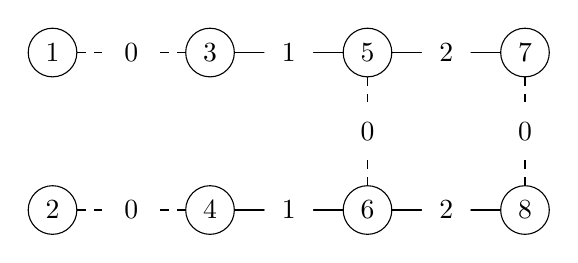
\begin{tikzpicture}

      \begin{scope}[every node/.style={circle,draw}]
        \node (1)  at (0,2)  {1};
        \node (2)  at (0,0)  {2};
        \node (3)  at (2,2)  {3};
        \node (4)  at (2,0)  {4};
        \node (5)  at (4,2)  {5};
        \node (6)  at (4,0)  {6};
        \node (7)  at (6,2)  {7};
        \node (8)  at (6,0)  {8};
      \end{scope}

      \begin{scope}[every node/.style={fill=white,circle}]

        \begin{scope}[every edge/.style={draw}]
          \path (3)  edge node {$1$} (5);
          \path (4)  edge node {$1$} (6);
          \path (5)  edge node {$2$} (7);
          \path (6)  edge node {$2$} (8);
        \end{scope}

        \begin{scope}[every edge/.style={draw,dashed}]
          \path (1)  edge node {$0$} (3);
          \path (2)  edge node {$0$} (4);
          \path (5)  edge node {$0$} (6);
          \path (7)  edge node {$0$} (8);
        \end{scope}

      \end{scope}

    \end{tikzpicture}
  \end{center}
  \caption{Degré huit, carré avec $\rho_0$ comme involution verticale}
  \label{f.d8.l0.l}
\end{figure}

\paragraph{}
Concernant le graphe \ref{f.d6.l2}, un raisonnement similaire nous donne le graphe \ref{f.d8.l2.l}


\begin{figure}[H]
  \begin{center}
    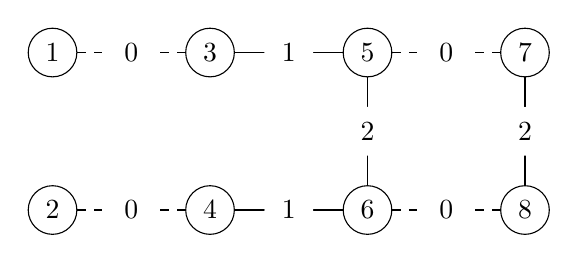
\begin{tikzpicture}

      \begin{scope}[every node/.style={circle,draw}]
        \node (1)  at (0,2)  {1};
        \node (2)  at (0,0)  {2};
        \node (3)  at (2,2)  {3};
        \node (4)  at (2,0)  {4};
        \node (5)  at (4,2)  {5};
        \node (6)  at (4,0)  {6};
        \node (7)  at (6,2)  {7};
        \node (8)  at (6,0)  {8};
      \end{scope}

      \begin{scope}[every node/.style={fill=white,circle}]

        \begin{scope}[every edge/.style={draw}]
          \path (3)  edge node {$1$} (5);
          \path (4)  edge node {$1$} (6);
          \path (5)  edge node {$2$} (6);
          \path (7)  edge node {$2$} (8);
        \end{scope}

        \begin{scope}[every edge/.style={draw,dashed}]
          \path (1)  edge node {$0$} (3);
          \path (2)  edge node {$0$} (4);
          \path (5)  edge node {$0$} (7);
          \path (6)  edge node {$0$} (8);
        \end{scope}

      \end{scope}

    \end{tikzpicture}
  \end{center}
  \caption{Degré huit, carré avec $\rho_2$ comme involution verticale}
  \label{f.d8.l2.l}
\end{figure}

\paragraph{}
Dans le cas du graphe \ref{f.d6.l02}, l'involution qui doit relier les points 5 et 7 doit être $\rho_0$ ou $\rho_2$ mais aucune des deux n'est possible car elles sont déjà utilisées pour relier le point 5 au point 6.

\paragraph{}
Concernant le dernier graphe, vu qu'il n'est pas connexe, on rajoute un point sur chaque ligne. On doit choisir parmi les involutions $\rho_0$ et $\rho_2$ ou les deux pour relier le point 5 au point 7. Idem pour les points 6 et 8. Ensuite, on peut relier les points 7 et 8 avec l'involution $\rho_1$ ou, dans certains cas, une nouvelle involution $\rho_3$. Nous allons énumérer toutes les possibilités (nous n'indiquerons pas les graphes qui ne sont qu'une permutation des deux lignes). On trouve les graphes entre \ref{f.d8.l.0.0} et \ref{f.d8.nl.02.02}.

\begin{figure}[H]
  \begin{center}
    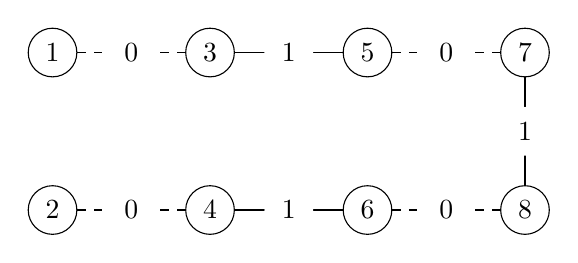
\begin{tikzpicture}

      \begin{scope}[every node/.style={circle,draw}]
        \node (1)  at (0,2)  {1};
        \node (2)  at (0,0)  {2};
        \node (3)  at (2,2)  {3};
        \node (4)  at (2,0)  {4};
        \node (5)  at (4,2)  {5};
        \node (6)  at (4,0)  {6};
        \node (7)  at (6,2)  {7};
        \node (8)  at (6,0)  {8};
      \end{scope}

      \begin{scope}[every node/.style={fill=white,circle}]

        \begin{scope}[every edge/.style={draw}]
          \path (3)  edge node {$1$} (5);
          \path (4)  edge node {$1$} (6);
          \path (7)  edge node {$1$} (8);
        \end{scope}

        \begin{scope}[every edge/.style={draw,dashed}]
          \path (1)  edge node {$0$} (3);
          \path (2)  edge node {$0$} (4);
          \path (5)  edge node {$0$} (7);
          \path (6)  edge node {$0$} (8);
        \end{scope}

      \end{scope}

    \end{tikzpicture}
  \end{center}
  \caption{Degré huit, reliés}
  \label{f.d8.l.0.0}
\end{figure}

\begin{figure}[H]
  \begin{center}
    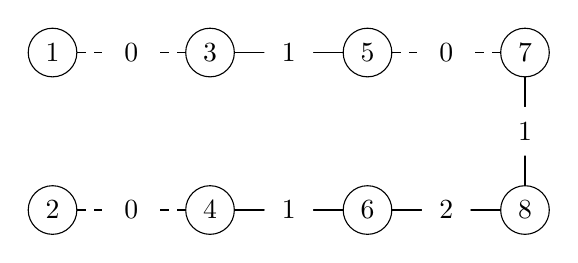
\begin{tikzpicture}

      \begin{scope}[every node/.style={circle,draw}]
        \node (1)  at (0,2)  {1};
        \node (2)  at (0,0)  {2};
        \node (3)  at (2,2)  {3};
        \node (4)  at (2,0)  {4};
        \node (5)  at (4,2)  {5};
        \node (6)  at (4,0)  {6};
        \node (7)  at (6,2)  {7};
        \node (8)  at (6,0)  {8};
      \end{scope}

      \begin{scope}[every node/.style={fill=white,circle}]

        \begin{scope}[every edge/.style={draw}]
          \path (3)  edge node {$1$} (5);
          \path (4)  edge node {$1$} (6);
          \path (6)  edge node {$2$} (8);
          \path (7)  edge node {$1$} (8);
        \end{scope}

        \begin{scope}[every edge/.style={draw,dashed}]
          \path (1)  edge node {$0$} (3);
          \path (2)  edge node {$0$} (4);
          \path (5)  edge node {$0$} (7);
        \end{scope}

      \end{scope}

    \end{tikzpicture}
  \end{center}
  \caption{Degré huit, reliés}
  \label{f.d8.l.0.2}
\end{figure}

\begin{figure}[H]
  \begin{center}
    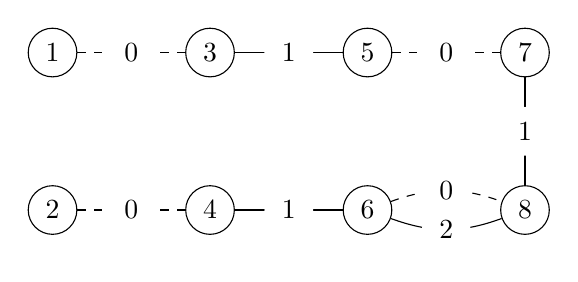
\begin{tikzpicture}

      \begin{scope}[every node/.style={circle,draw}]
        \node (1)  at (0,2)  {1};
        \node (2)  at (0,0)  {2};
        \node (3)  at (2,2)  {3};
        \node (4)  at (2,0)  {4};
        \node (5)  at (4,2)  {5};
        \node (6)  at (4,0)  {6};
        \node (7)  at (6,2)  {7};
        \node (8)  at (6,0)  {8};
      \end{scope}

      \begin{scope}[every node/.style={fill=white,circle}]

        \begin{scope}[every edge/.style={draw}]
          \path (3)  edge node {$1$} (5);
          \path (4)  edge node {$1$} (6);
          \path (6)  edge[bend right=20] node {$2$} (8);
          \path (7)  edge node {$1$} (8);
        \end{scope}

        \begin{scope}[every edge/.style={draw,dashed}]
          \path (1)  edge node {$0$} (3);
          \path (2)  edge node {$0$} (4);
          \path (5)  edge node {$0$} (7);
          \path (6)  edge[bend left=20] node {$0$} (8);
        \end{scope}

      \end{scope}

    \end{tikzpicture}
  \end{center}
  \caption{Degré huit, reliés}
  \label{f.d8.l.0.02}
\end{figure}

\begin{figure}[H]
  \begin{center}
    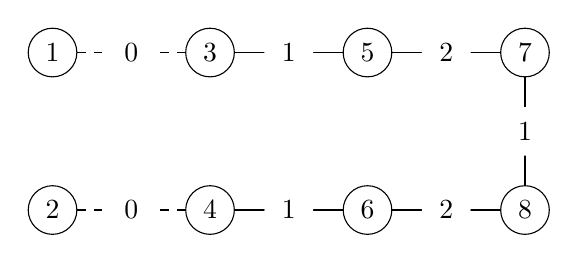
\begin{tikzpicture}

      \begin{scope}[every node/.style={circle,draw}]
        \node (1)  at (0,2)  {1};
        \node (2)  at (0,0)  {2};
        \node (3)  at (2,2)  {3};
        \node (4)  at (2,0)  {4};
        \node (5)  at (4,2)  {5};
        \node (6)  at (4,0)  {6};
        \node (7)  at (6,2)  {7};
        \node (8)  at (6,0)  {8};
      \end{scope}

      \begin{scope}[every node/.style={fill=white,circle}]

        \begin{scope}[every edge/.style={draw}]
          \path (3)  edge node {$1$} (5);
          \path (4)  edge node {$1$} (6);
          \path (5)  edge node {$2$} (7);
          \path (6)  edge node {$2$} (8);
          \path (7)  edge node {$1$} (8);
        \end{scope}

        \begin{scope}[every edge/.style={draw,dashed}]
          \path (1)  edge node {$0$} (3);
          \path (2)  edge node {$0$} (4);
        \end{scope}

      \end{scope}

    \end{tikzpicture}
  \end{center}
  \caption{Degré huit, reliés}
  \label{f.d8.l.2.2}
\end{figure}

\begin{figure}[H]
  \begin{center}
    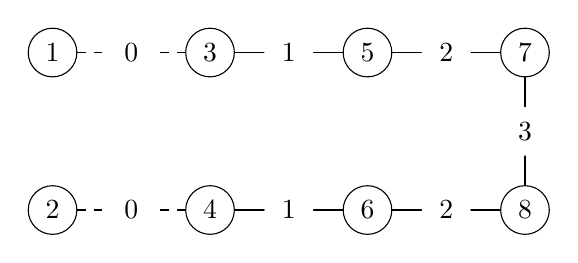
\begin{tikzpicture}

      \begin{scope}[every node/.style={circle,draw}]
        \node (1)  at (0,2)  {1};
        \node (2)  at (0,0)  {2};
        \node (3)  at (2,2)  {3};
        \node (4)  at (2,0)  {4};
        \node (5)  at (4,2)  {5};
        \node (6)  at (4,0)  {6};
        \node (7)  at (6,2)  {7};
        \node (8)  at (6,0)  {8};
      \end{scope}

      \begin{scope}[every node/.style={fill=white,circle}]

        \begin{scope}[every edge/.style={draw}]
          \path (3)  edge node {$1$} (5);
          \path (4)  edge node {$1$} (6);
          \path (7)  edge node {$3$} (8);
          \path (5)  edge node {$2$} (7);
          \path (6)  edge node {$2$} (8);
        \end{scope}

        \begin{scope}[every edge/.style={draw,dashed}]
          \path (1)  edge node {$0$} (3);
          \path (2)  edge node {$0$} (4);

        \end{scope}

      \end{scope}

    \end{tikzpicture}
  \end{center}
  \caption{Degré huit, reliés avec $\rho_3$}
  \label{f.d8.lb.2.2}
\end{figure}

\begin{figure}[H]
  \begin{center}
    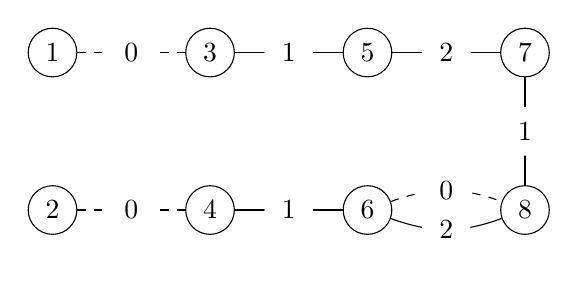
\begin{tikzpicture}

      \begin{scope}[every node/.style={circle,draw}]
        \node (1)  at (0,2)  {1};
        \node (2)  at (0,0)  {2};
        \node (3)  at (2,2)  {3};
        \node (4)  at (2,0)  {4};
        \node (5)  at (4,2)  {5};
        \node (6)  at (4,0)  {6};
        \node (7)  at (6,2)  {7};
        \node (8)  at (6,0)  {8};
      \end{scope}

      \begin{scope}[every node/.style={fill=white,circle}]

        \begin{scope}[every edge/.style={draw}]
          \path (3)  edge node {$1$} (5);
          \path (4)  edge node {$1$} (6);
          \path (5)  edge node {$2$} (7);
          \path (6)  edge[bend right=20] node {$2$} (8);
          \path (7)  edge node {$1$} (8);
        \end{scope}

        \begin{scope}[every edge/.style={draw,dashed}]
          \path (1)  edge node {$0$} (3);
          \path (2)  edge node {$0$} (4);
          \path (6)  edge[bend left=20] node {$0$} (8);
        \end{scope}

      \end{scope}

    \end{tikzpicture}
  \end{center}
  \caption{Degré huit, reliés}
  \label{f.d8.l.2.02}
\end{figure}

\begin{figure}[H]
  \begin{center}
    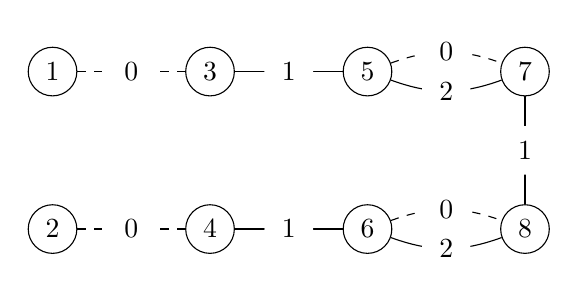
\begin{tikzpicture}

      \begin{scope}[every node/.style={circle,draw}]
        \node (1)  at (0,2)  {1};
        \node (2)  at (0,0)  {2};
        \node (3)  at (2,2)  {3};
        \node (4)  at (2,0)  {4};
        \node (5)  at (4,2)  {5};
        \node (6)  at (4,0)  {6};
        \node (7)  at (6,2)  {7};
        \node (8)  at (6,0)  {8};
      \end{scope}

      \begin{scope}[every node/.style={fill=white,circle}]

        \begin{scope}[every edge/.style={draw}]
          \path (3)  edge node {$1$} (5);
          \path (4)  edge node {$1$} (6);
          \path (5)  edge[bend right=20] node {$2$} (7);
          \path (6)  edge[bend right=20] node {$2$} (8);
          \path (7)  edge node {$1$} (8);
        \end{scope}

        \begin{scope}[every edge/.style={draw,dashed}]
          \path (1)  edge node {$0$} (3);
          \path (2)  edge node {$0$} (4);
          \path (5)  edge[bend left=20] node {$0$} (7);
          \path (6)  edge[bend left=20] node {$0$} (8);
        \end{scope}

      \end{scope}

    \end{tikzpicture}
  \end{center}
  \caption{Degré huit, reliés}
  \label{f.d8.l.02.02}
\end{figure}

\begin{figure}[H]
  \begin{center}
    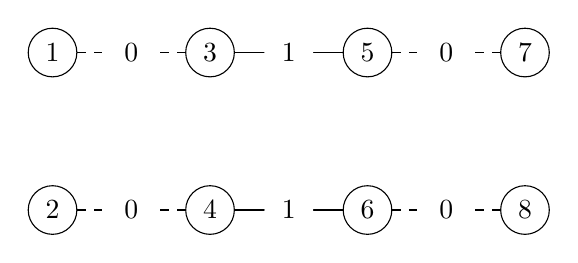
\begin{tikzpicture}

      \begin{scope}[every node/.style={circle,draw}]
        \node (1)  at (0,2)  {1};
        \node (2)  at (0,0)  {2};
        \node (3)  at (2,2)  {3};
        \node (4)  at (2,0)  {4};
        \node (5)  at (4,2)  {5};
        \node (6)  at (4,0)  {6};
        \node (7)  at (6,2)  {7};
        \node (8)  at (6,0)  {8};
      \end{scope}

      \begin{scope}[every node/.style={fill=white,circle}]

        \begin{scope}[every edge/.style={draw}]
          \path (3)  edge node {$1$} (5);
          \path (4)  edge node {$1$} (6);
        \end{scope}

        \begin{scope}[every edge/.style={draw,dashed}]
          \path (1)  edge node {$0$} (3);
          \path (2)  edge node {$0$} (4);
          \path (5)  edge node {$0$} (7);
          \path (6)  edge node {$0$} (8);
        \end{scope}

      \end{scope}

    \end{tikzpicture}
  \end{center}
  \caption{Degré huit, non reliés}
  \label{f.d8.nl.0.0}
\end{figure}

\begin{figure}[H]
  \begin{center}
    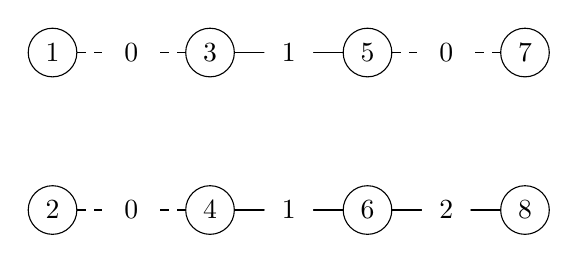
\begin{tikzpicture}

      \begin{scope}[every node/.style={circle,draw}]
        \node (1)  at (0,2)  {1};
        \node (2)  at (0,0)  {2};
        \node (3)  at (2,2)  {3};
        \node (4)  at (2,0)  {4};
        \node (5)  at (4,2)  {5};
        \node (6)  at (4,0)  {6};
        \node (7)  at (6,2)  {7};
        \node (8)  at (6,0)  {8};
      \end{scope}

      \begin{scope}[every node/.style={fill=white,circle}]

        \begin{scope}[every edge/.style={draw}]
          \path (3)  edge node {$1$} (5);
          \path (4)  edge node {$1$} (6);
          \path (6)  edge node {$2$} (8);
        \end{scope}

        \begin{scope}[every edge/.style={draw,dashed}]
          \path (1)  edge node {$0$} (3);
          \path (2)  edge node {$0$} (4);
          \path (5)  edge node {$0$} (7);
        \end{scope}

      \end{scope}

    \end{tikzpicture}
  \end{center}
  \caption{Degré huit, non reliés}
  \label{f.d8.nl.0.2}
\end{figure}

\begin{figure}[H]
  \begin{center}
    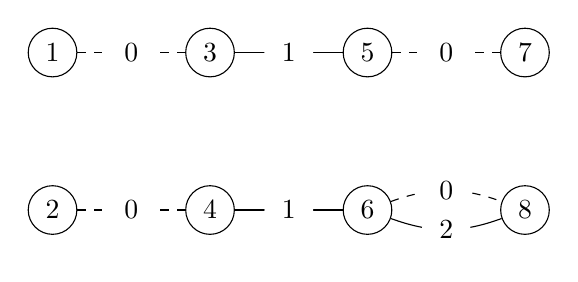
\begin{tikzpicture}

      \begin{scope}[every node/.style={circle,draw}]
        \node (1)  at (0,2)  {1};
        \node (2)  at (0,0)  {2};
        \node (3)  at (2,2)  {3};
        \node (4)  at (2,0)  {4};
        \node (5)  at (4,2)  {5};
        \node (6)  at (4,0)  {6};
        \node (7)  at (6,2)  {7};
        \node (8)  at (6,0)  {8};
      \end{scope}

      \begin{scope}[every node/.style={fill=white,circle}]

        \begin{scope}[every edge/.style={draw}]
          \path (3)  edge node {$1$} (5);
          \path (4)  edge node {$1$} (6);
          \path (6)  edge[bend right=20] node {$2$} (8);
        \end{scope}

        \begin{scope}[every edge/.style={draw,dashed}]
          \path (1)  edge node {$0$} (3);
          \path (2)  edge node {$0$} (4);
          \path (5)  edge node {$0$} (7);
          \path (6)  edge[bend left=20] node {$0$} (8);
        \end{scope}

      \end{scope}

    \end{tikzpicture}
  \end{center}
  \caption{Degré huit, non reliés}
  \label{f.d8.nl.0.02}
\end{figure}

\begin{figure}[H]
  \begin{center}
    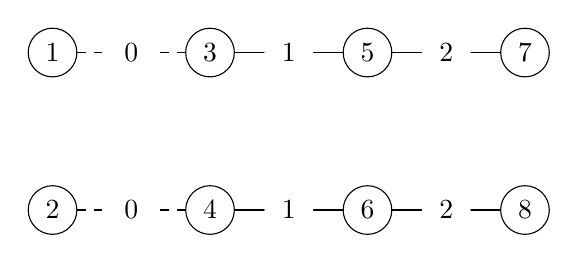
\begin{tikzpicture}

      \begin{scope}[every node/.style={circle,draw}]
        \node (1)  at (0,2)  {1};
        \node (2)  at (0,0)  {2};
        \node (3)  at (2,2)  {3};
        \node (4)  at (2,0)  {4};
        \node (5)  at (4,2)  {5};
        \node (6)  at (4,0)  {6};
        \node (7)  at (6,2)  {7};
        \node (8)  at (6,0)  {8};
      \end{scope}

      \begin{scope}[every node/.style={fill=white,circle}]

        \begin{scope}[every edge/.style={draw}]
          \path (3)  edge node {$1$} (5);
          \path (4)  edge node {$1$} (6);
          \path (5)  edge node {$2$} (7);
          \path (6)  edge node {$2$} (8);
        \end{scope}

        \begin{scope}[every edge/.style={draw,dashed}]
          \path (1)  edge node {$0$} (3);
          \path (2)  edge node {$0$} (4);
        \end{scope}

      \end{scope}

    \end{tikzpicture}
  \end{center}
  \caption{Degré huit, non reliés}
  \label{f.d8.nl.2.2}
\end{figure}

\begin{figure}[H]
  \begin{center}
    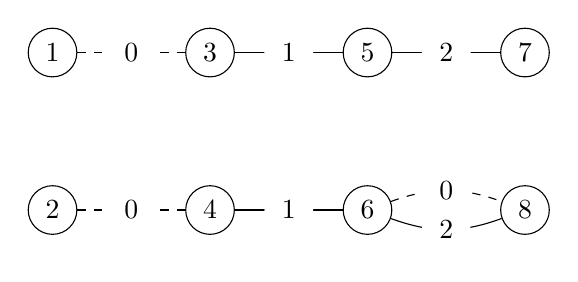
\begin{tikzpicture}

      \begin{scope}[every node/.style={circle,draw}]
        \node (1)  at (0,2)  {1};
        \node (2)  at (0,0)  {2};
        \node (3)  at (2,2)  {3};
        \node (4)  at (2,0)  {4};
        \node (5)  at (4,2)  {5};
        \node (6)  at (4,0)  {6};
        \node (7)  at (6,2)  {7};
        \node (8)  at (6,0)  {8};
      \end{scope}

      \begin{scope}[every node/.style={fill=white,circle}]

        \begin{scope}[every edge/.style={draw}]
          \path (3)  edge node {$1$} (5);
          \path (4)  edge node {$1$} (6);
          \path (5)  edge node {$2$} (7);
          \path (6)  edge[bend right=20] node {$2$} (8);
        \end{scope}

        \begin{scope}[every edge/.style={draw,dashed}]
          \path (1)  edge node {$0$} (3);
          \path (2)  edge node {$0$} (4);
          \path (6)  edge[bend left=20] node {$0$} (8);
        \end{scope}

      \end{scope}

    \end{tikzpicture}
  \end{center}
  \caption{Degré huit, non reliés}
  \label{f.d8.nl.2.02}
\end{figure}

\begin{figure}[H]
  \begin{center}
    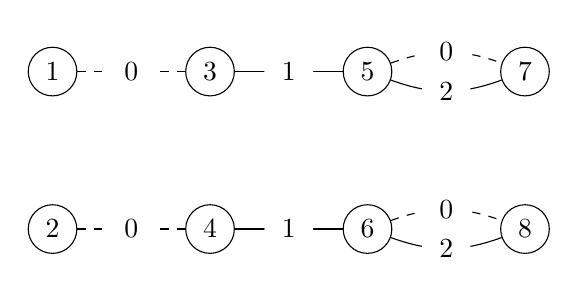
\begin{tikzpicture}

      \begin{scope}[every node/.style={circle,draw}]
        \node (1)  at (0,2)  {1};
        \node (2)  at (0,0)  {2};
        \node (3)  at (2,2)  {3};
        \node (4)  at (2,0)  {4};
        \node (5)  at (4,2)  {5};
        \node (6)  at (4,0)  {6};
        \node (7)  at (6,2)  {7};
        \node (8)  at (6,0)  {8};
      \end{scope}

      \begin{scope}[every node/.style={fill=white,circle}]

        \begin{scope}[every edge/.style={draw}]
          \path (3)  edge node {$1$} (5);
          \path (4)  edge node {$1$} (6);
          \path (5)  edge[bend right=20] node {$2$} (7);
          \path (6)  edge[bend right=20] node {$2$} (8);
        \end{scope}

        \begin{scope}[every edge/.style={draw,dashed}]
          \path (1)  edge node {$0$} (3);
          \path (2)  edge node {$0$} (4);
          \path (5)  edge[bend left=20] node {$0$} (7);
          \path (6)  edge[bend left=20] node {$0$} (8);
        \end{scope}

      \end{scope}

    \end{tikzpicture}
  \end{center}
  \caption{Degré huit, non reliés}
  \label{f.d8.nl.02.02}
\end{figure}

\subsection{Degré 9}

\paragraph{}
Pour les graphes \ref{f.d8.l0.l} et \ref{f.d8.l2.l}, nous pouvons utiliser le lemme \ref{attachEven}

\paragraph{}
Pour les graphes \ref{f.d8.l.0.0}, \ref{f.d8.l.0.2}, \ref{f.d8.l.0.02}, \ref{f.d8.l.2.2}, \ref{f.d8.l.2.02} et \ref{f.d8.l.02.02}, nous pouvons utiliser le lemme \ref{attachNoFixedPoint} sur l'involution $\rho_0$.

\paragraph{}
Pour le graphes \ref{f.d8.lb.2.2}, il faut utiliser le lemme \ref{attachNoFixedPoint} sur $\rho_3$.

\paragraph{}
Pour le graphes \ref{f.d8.nl.0.0}, \ref{f.d8.nl.0.02}, \ref{f.d8.nl.2.2}, \ref{f.d8.nl.2.02} et \ref{f.d8.nl.02.02}, on peut conclure en utilisant le lemme \ref{attachConnexEven}.

\paragraph{}
Dans le cas du graphe~\ref{f.d8.nl.2.2}, on doit atache le sommet supplémentaire en utilisant les involutions $\rho_0$ et $\rho_2$. Mais les involutions ne sont pas consécutives donc on a un problème sur le sommet supplementaire.

\subsection{Degré 10}

\paragraph{}
Essayons d'étendre le graphe \ref{f.d8.l0.l}, il nous faut relier les sommet 7 et 9, nous avons le choix entre l'involution $\rho_1$ ou $\rho_3$. Dans le cas de $\rho_3$, il faut faire un carré qui doit venir se connecter sur le point 8.

\begin{figure}[H]
  \begin{center}
    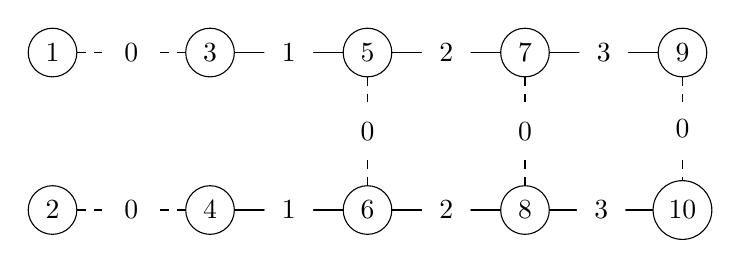
\begin{tikzpicture}

      \begin{scope}[every node/.style={circle,draw}]
        \node (1)  at (0,2)  {1};
        \node (2)  at (0,0)  {2};
        \node (3)  at (2,2)  {3};
        \node (4)  at (2,0)  {4};
        \node (5)  at (4,2)  {5};
        \node (6)  at (4,0)  {6};
        \node (7)  at (6,2)  {7};
        \node (8)  at (6,0)  {8};
        \node (9)  at (8,2)  {9};
        \node (10) at (8,0)  {10};
      \end{scope}

      \begin{scope}[every node/.style={fill=white,circle}]

        \begin{scope}[every edge/.style={draw}]
          \path (3)  edge node {$1$} (5);
          \path (4)  edge node {$1$} (6);
          \path (5)  edge node {$2$} (7);
          \path (6)  edge node {$2$} (8);
          \path (7)  edge node {$3$} (9);
          \path (8)  edge node {$3$} (10);
        \end{scope}

        \begin{scope}[every edge/.style={draw,dashed}]
          \path (1)  edge node {$0$} (3);
          \path (2)  edge node {$0$} (4);
          \path (5)  edge node {$0$} (6);
          \path (7)  edge node {$0$} (8);
          \path (9)  edge node {$0$} (10);
        \end{scope}

      \end{scope}

    \end{tikzpicture}
  \end{center}
  \caption{Degré 10, carré avec $\rho_0$ comme involution verticale, un point par ligne, avec une involution $\rho_3$}
  \label{f.d10.l0.l3}
\end{figure}

\begin{figure}[H]
  \begin{center}
    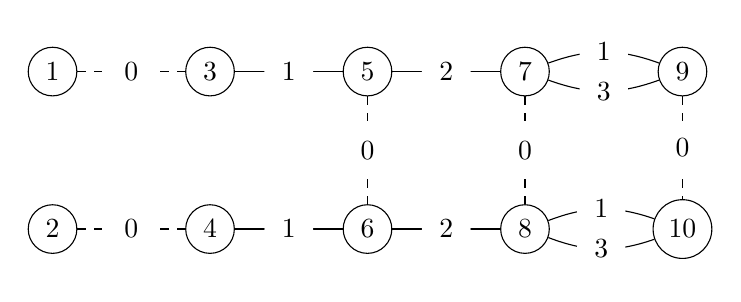
\begin{tikzpicture}

      \begin{scope}[every node/.style={circle,draw}]
        \node (1)  at (0,2)  {1};
        \node (2)  at (0,0)  {2};
        \node (3)  at (2,2)  {3};
        \node (4)  at (2,0)  {4};
        \node (5)  at (4,2)  {5};
        \node (6)  at (4,0)  {6};
        \node (7)  at (6,2)  {7};
        \node (8)  at (6,0)  {8};
        \node (9)  at (8,2)  {9};
        \node (10) at (8,0)  {10};
      \end{scope}

      \begin{scope}[every node/.style={fill=white,circle}]

        \begin{scope}[every edge/.style={draw}]
          \path (3)  edge node {$1$} (5);
          \path (4)  edge node {$1$} (6);
          \path (5)  edge node {$2$} (7);
          \path (6)  edge node {$2$} (8);
          \path (7)  edge[bend left=20] node {$1$} (9);
          \path (8)  edge[bend left=20] node {$1$} (10);
          \path (7)  edge[bend right=20] node {$3$} (9);
          \path (8)  edge[bend right=20] node {$3$} (10);
        \end{scope}

        \begin{scope}[every edge/.style={draw,dashed}]
          \path (1)  edge node {$0$} (3);
          \path (2)  edge node {$0$} (4);
          \path (5)  edge node {$0$} (6);
          \path (7)  edge node {$0$} (8);
          \path (9)  edge node {$0$} (10);
        \end{scope}

      \end{scope}

    \end{tikzpicture}
  \end{center}
  \caption{Degré 10, carré avec $\rho_0$ comme involution verticale, un point par ligne, avec une involution $\rho_3$}
  \label{f.d10.l0.l13}
\end{figure}

\paragraph{}
Si nous utilisons l'involution $\rho_0$, nous avons deux possibilités pour le point 10. Soit nous le relions avec 8, toujours en utilisant l'involution $\rho_1$ et puis nous avons le choix quant à la manière de relier les point 9 et 10. Soit nous ne relions pas 8 et 10 et nous devons alors relier 10 à 9 car c'est impossible pour les points 5, 6 et 7. Là encore nous avons le choix quant à la manière de réaliser le lien entre 9 et 10. On trouve donc les graphes

\begin{figure}[H]
  \begin{center}
    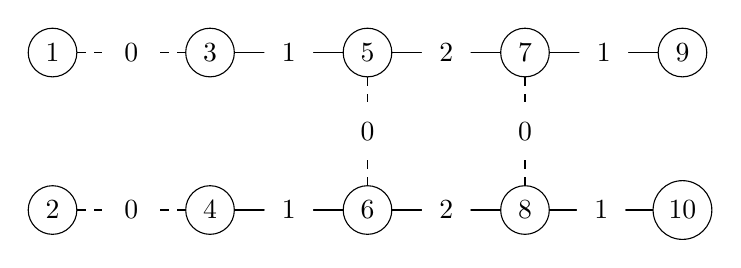
\begin{tikzpicture}

      \begin{scope}[every node/.style={circle,draw}]
        \node (1)  at (0,2)  {1};
        \node (2)  at (0,0)  {2};
        \node (3)  at (2,2)  {3};
        \node (4)  at (2,0)  {4};
        \node (5)  at (4,2)  {5};
        \node (6)  at (4,0)  {6};
        \node (7)  at (6,2)  {7};
        \node (8)  at (6,0)  {8};
        \node (9)  at (8,2)  {9};
        \node (10) at (8,0)  {10};
      \end{scope}

      \begin{scope}[every node/.style={fill=white,circle}]

        \begin{scope}[every edge/.style={draw}]
          \path (3)  edge node {$1$} (5);
          \path (4)  edge node {$1$} (6);
          \path (5)  edge node {$2$} (7);
          \path (6)  edge node {$2$} (8);
          \path (7)  edge node {$1$} (9);
          \path (8)  edge node {$1$} (10);
        \end{scope}

        \begin{scope}[every edge/.style={draw,dashed}]
          \path (1)  edge node {$0$} (3);
          \path (2)  edge node {$0$} (4);
          \path (5)  edge node {$0$} (6);
          \path (7)  edge node {$0$} (8);
        \end{scope}

      \end{scope}

    \end{tikzpicture}
  \end{center}
  \caption{Degré 10, carré avec $\rho_0$ comme involution verticale, un point par ligne, non-reliés}
  \label{f.d10.l0.l.c.nl}
\end{figure}

\begin{figure}[H]
  \begin{center}
    \begin{tikzpicture}

      \begin{scope}[every node/.style={circle,draw}]
        \node (1)  at (0,2)  {1};
        \node (2)  at (0,0)  {2};
        \node (3)  at (2,2)  {3};
        \node (4)  at (2,0)  {4};
        \node (5)  at (4,2)  {5};
        \node (6)  at (4,0)  {6};
        \node (7)  at (6,2)  {7};
        \node (8)  at (6,0)  {8};
        \node (9)  at (8,2)  {9};
        \node (10) at (8,0)  {10};
      \end{scope}

      \begin{scope}[every node/.style={fill=white,circle}]

        \begin{scope}[every edge/.style={draw}]
          \path (3)  edge node {$1$} (5);
          \path (4)  edge node {$1$} (6);
          \path (5)  edge node {$2$} (7);
          \path (6)  edge node {$2$} (8);
          \path (7)  edge node {$1$} (9);
          \path (8)  edge node {$1$} (10);
        \end{scope}

        \begin{scope}[every edge/.style={draw,dashed}]
          \path (1)  edge node {$0$} (3);
          \path (2)  edge node {$0$} (4);
          \path (5)  edge node {$0$} (6);
          \path (7)  edge node {$0$} (8);
          \path (9)  edge node {$0$} (10);
        \end{scope}

      \end{scope}

    \end{tikzpicture}
  \end{center}
  \caption{Degré 10, carré avec $\rho_0$ comme involution verticale, un point par ligne, reliés par $\rho_0$}
  \label{f.d10.l0.l.c.l.0}
\end{figure}

\begin{figure}[H]
  \begin{center}
    \begin{tikzpicture}

      \begin{scope}[every node/.style={circle,draw}]
        \node (1)  at (0,2)  {1};
        \node (2)  at (0,0)  {2};
        \node (3)  at (2,2)  {3};
        \node (4)  at (2,0)  {4};
        \node (5)  at (4,2)  {5};
        \node (6)  at (4,0)  {6};
        \node (7)  at (6,2)  {7};
        \node (8)  at (6,0)  {8};
        \node (9)  at (8,2)  {9};
        \node (10) at (8,0)  {10};
      \end{scope}

      \begin{scope}[every node/.style={fill=white,circle}]

        \begin{scope}[every edge/.style={draw}]
          \path (3)  edge node {$1$} (5);
          \path (4)  edge node {$1$} (6);
          \path (5)  edge node {$2$} (7);
          \path (6)  edge node {$2$} (8);
          \path (7)  edge node {$1$} (9);
          \path (8)  edge node {$1$} (10);
          \path (9)  edge node {$2$} (10);
        \end{scope}

        \begin{scope}[every edge/.style={draw,dashed}]
          \path (1)  edge node {$0$} (3);
          \path (2)  edge node {$0$} (4);
          \path (5)  edge node {$0$} (6);
          \path (7)  edge node {$0$} (8);
        \end{scope}

      \end{scope}

    \end{tikzpicture}
  \end{center}
  \caption{Degré 10, carré avec $\rho_0$ comme involution verticale, un point par ligne, reliés par $\rho_2$}
  \label{f.d10.l0.l.c.l.2}
\end{figure}


\begin{figure}[H]
  \begin{center}
    \begin{tikzpicture}

      \begin{scope}[every node/.style={circle,draw}]
        \node (1)  at (0,2)  {1};
        \node (2)  at (0,0)  {2};
        \node (3)  at (2,2)  {3};
        \node (4)  at (2,0)  {4};
        \node (5)  at (4,2)  {5};
        \node (6)  at (4,0)  {6};
        \node (7)  at (6,2)  {7};
        \node (8)  at (6,0)  {8};
        \node (9)  at (8,2)  {9};
        \node (10) at (8,0)  {10};
      \end{scope}

      \begin{scope}[every node/.style={fill=white,circle}]

        \begin{scope}[every edge/.style={draw}]
          \path (3)  edge node {$1$} (5);
          \path (4)  edge node {$1$} (6);
          \path (5)  edge node {$2$} (7);
          \path (6)  edge node {$2$} (8);
          \path (7)  edge node {$1$} (9);
          \path (8)  edge node {$1$} (10);
          \path (9)  edge[bend left=20] node {$2$} (10);
        \end{scope}

        \begin{scope}[every edge/.style={draw,dashed}]
          \path (1)  edge node {$0$} (3);
          \path (2)  edge node {$0$} (4);
          \path (5)  edge node {$0$} (6);
          \path (7)  edge node {$0$} (8);
          \path (9)  edge[bend right=20] node {$0$} (10);
        \end{scope}

      \end{scope}

    \end{tikzpicture}
  \end{center}
  \caption{Degré 10, carré avec $\rho_0$ comme involution verticale, un point par ligne, reliés par $\rho_0$ et $\rho_2$}
  \label{f.d10.l0.l.c.l.02}
\end{figure}

\begin{figure}[H]
  \begin{center}
    \begin{tikzpicture}

      \begin{scope}[every node/.style={circle,draw}]
        \node (1)  at (0,2)  {1};
        \node (2)  at (0,0)  {2};
        \node (3)  at (2,2)  {3};
        \node (4)  at (2,0)  {4};
        \node (5)  at (4,2)  {5};
        \node (6)  at (4,0)  {6};
        \node (7)  at (6,2)  {7};
        \node (8)  at (6,0)  {8};
        \node (9)  at (8,2)  {9};
        \node (10) at (10,2) {10};
      \end{scope}

      \begin{scope}[every node/.style={fill=white,circle}]

        \begin{scope}[every edge/.style={draw}]
          \path (3)  edge node {$1$} (5);
          \path (4)  edge node {$1$} (6);
          \path (5)  edge node {$2$} (7);
          \path (6)  edge node {$2$} (8);
          \path (7)  edge node {$1$} (9);
        \end{scope}

        \begin{scope}[every edge/.style={draw,dashed}]
          \path (1)  edge node {$0$} (3);
          \path (2)  edge node {$0$} (4);
          \path (5)  edge node {$0$} (6);
          \path (7)  edge node {$0$} (8);
          \path (9)  edge node {$0$} (10);
        \end{scope}

      \end{scope}

    \end{tikzpicture}
  \end{center}
  \caption{Degré 10, carré avec $\rho_0$ comme involution verticale, un point par ligne, reliés par $\rho_0$}
  \label{f.d10.l0.l.0}
\end{figure}

\begin{figure}[H]
  \begin{center}
    \begin{tikzpicture}

      \begin{scope}[every node/.style={circle,draw}]
        \node (1)  at (0,2)  {1};
        \node (2)  at (0,0)  {2};
        \node (3)  at (2,2)  {3};
        \node (4)  at (2,0)  {4};
        \node (5)  at (4,2)  {5};
        \node (6)  at (4,0)  {6};
        \node (7)  at (6,2)  {7};
        \node (8)  at (6,0)  {8};
        \node (9)  at (8,2)  {9};
        \node (10) at (10,2) {10};
      \end{scope}

      \begin{scope}[every node/.style={fill=white,circle}]

        \begin{scope}[every edge/.style={draw}]
          \path (3)  edge node {$1$} (5);
          \path (4)  edge node {$1$} (6);
          \path (5)  edge node {$2$} (7);
          \path (6)  edge node {$2$} (8);
          \path (7)  edge node {$1$} (9);
          \path (9)  edge node {$2$} (10);
        \end{scope}

        \begin{scope}[every edge/.style={draw,dashed}]
          \path (1)  edge node {$0$} (3);
          \path (2)  edge node {$0$} (4);
          \path (5)  edge node {$0$} (6);
          \path (7)  edge node {$0$} (8);
        \end{scope}

      \end{scope}

    \end{tikzpicture}
  \end{center}
  \caption{Degré 10, carré avec $\rho_0$ comme involution verticale, un point par ligne, reliés par $\rho_2$}
  \label{f.d10.l0.l.2}
\end{figure}


\begin{figure}[H]
  \begin{center}
    \begin{tikzpicture}

      \begin{scope}[every node/.style={circle,draw}]
        \node (1)  at (0,2)  {1};
        \node (2)  at (0,0)  {2};
        \node (3)  at (2,2)  {3};
        \node (4)  at (2,0)  {4};
        \node (5)  at (4,2)  {5};
        \node (6)  at (4,0)  {6};
        \node (7)  at (6,2)  {7};
        \node (8)  at (6,0)  {8};
        \node (9)  at (8,2)  {9};
        \node (10) at (10,2) {10};
      \end{scope}

      \begin{scope}[every node/.style={fill=white,circle}]

        \begin{scope}[every edge/.style={draw}]
          \path (3)  edge node {$1$} (5);
          \path (4)  edge node {$1$} (6);
          \path (5)  edge node {$2$} (7);
          \path (6)  edge node {$2$} (8);
          \path (7)  edge node {$1$} (9);
          \path (9)  edge[bend right=20] node {$2$} (10);
        \end{scope}

        \begin{scope}[every edge/.style={draw,dashed}]
          \path (1)  edge node {$0$} (3);
          \path (2)  edge node {$0$} (4);
          \path (5)  edge node {$0$} (6);
          \path (7)  edge node {$0$} (8);
          \path (9)  edge[bend left=20] node {$0$} (10);
        \end{scope}

      \end{scope}

    \end{tikzpicture}
  \end{center}
  \caption{Degré 10, carré avec $\rho_0$ comme involution verticale, un point par ligne, reliés par $\rho_0$ et $\rho_2$}
  \label{f.d10.l0.l.l.02}
\end{figure}



\paragraph{}
On obtient presque le même résultat pour les extensions du graphe \ref{f.d8.l2.l}, il faut juste retirer les cas où l'on utilise l'involution $\rho_3$ pour relier 7 et 9 car pour former le carré il faudrait revenir sur le sommet 5 avec l'involution $\rho_1$, ce qui est impossible. On a donc que les possibilités


\begin{figure}[H]
  \begin{center}
    \begin{tikzpicture}

      \begin{scope}[every node/.style={circle,draw}]
        \node (1)  at (0,2)  {1};
        \node (2)  at (0,0)  {2};
        \node (3)  at (2,2)  {3};
        \node (4)  at (2,0)  {4};
        \node (5)  at (4,2)  {5};
        \node (6)  at (4,0)  {6};
        \node (7)  at (6,2)  {7};
        \node (8)  at (6,0)  {8};
        \node (9)  at (8,2)  {9};
        \node (10) at (8,0)  {10};
      \end{scope}

      \begin{scope}[every node/.style={fill=white,circle}]

        \begin{scope}[every edge/.style={draw}]
          \path (3)  edge node {$1$} (5);
          \path (4)  edge node {$1$} (6);
          \path (5)  edge node {$2$} (6);
          \path (7)  edge node {$2$} (8);
          \path (7)  edge node {$1$} (9);
          \path (8)  edge node {$1$} (10);
        \end{scope}

        \begin{scope}[every edge/.style={draw,dashed}]
          \path (1)  edge node {$0$} (3);
          \path (2)  edge node {$0$} (4);
          \path (5)  edge node {$0$} (7);
          \path (6)  edge node {$0$} (8);
        \end{scope}

      \end{scope}

    \end{tikzpicture}
  \end{center}
  \caption{Degré 10, carré avec $\rho_2$ comme involution verticale, un point par ligne, non-reliés}
  \label{f.d10.l2.l.c.nl}
\end{figure}

\begin{figure}[H]
  \begin{center}
    \begin{tikzpicture}

      \begin{scope}[every node/.style={circle,draw}]
        \node (1)  at (0,2)  {1};
        \node (2)  at (0,0)  {2};
        \node (3)  at (2,2)  {3};
        \node (4)  at (2,0)  {4};
        \node (5)  at (4,2)  {5};
        \node (6)  at (4,0)  {6};
        \node (7)  at (6,2)  {7};
        \node (8)  at (6,0)  {8};
        \node (9)  at (8,2)  {9};
        \node (10) at (8,0)  {10};
      \end{scope}

      \begin{scope}[every node/.style={fill=white,circle}]

        \begin{scope}[every edge/.style={draw}]
          \path (3)  edge node {$1$} (5);
          \path (4)  edge node {$1$} (6);
          \path (5)  edge node {$2$} (6);
          \path (7)  edge node {$2$} (8);
          \path (7)  edge node {$1$} (9);
          \path (8)  edge node {$1$} (10);
        \end{scope}

        \begin{scope}[every edge/.style={draw,dashed}]
          \path (1)  edge node {$0$} (3);
          \path (2)  edge node {$0$} (4);
          \path (5)  edge node {$0$} (7);
          \path (6)  edge node {$0$} (8);
          \path (9)  edge node {$0$} (10);
        \end{scope}

      \end{scope}

    \end{tikzpicture}
  \end{center}
  \caption{Degré 10, carré avec $\rho_2$ comme involution verticale, un point par ligne, reliés par $\rho_0$}
  \label{f.d10.l2.l.c.l.0}
\end{figure}

\begin{figure}[H]
  \begin{center}
    \begin{tikzpicture}

      \begin{scope}[every node/.style={circle,draw}]
        \node (1)  at (0,2)  {1};
        \node (2)  at (0,0)  {2};
        \node (3)  at (2,2)  {3};
        \node (4)  at (2,0)  {4};
        \node (5)  at (4,2)  {5};
        \node (6)  at (4,0)  {6};
        \node (7)  at (6,2)  {7};
        \node (8)  at (6,0)  {8};
        \node (9)  at (8,2)  {9};
        \node (10) at (8,0)  {10};
      \end{scope}

      \begin{scope}[every node/.style={fill=white,circle}]

        \begin{scope}[every edge/.style={draw}]
          \path (3)  edge node {$1$} (5);
          \path (4)  edge node {$1$} (6);
          \path (5)  edge node {$2$} (6);
          \path (7)  edge node {$2$} (8);
          \path (7)  edge node {$1$} (9);
          \path (8)  edge node {$1$} (10);
          \path (9)  edge node {$2$} (10);
        \end{scope}

        \begin{scope}[every edge/.style={draw,dashed}]
          \path (1)  edge node {$0$} (3);
          \path (2)  edge node {$0$} (4);
          \path (5)  edge node {$0$} (7);
          \path (6)  edge node {$0$} (8);
        \end{scope}

      \end{scope}

    \end{tikzpicture}
  \end{center}
  \caption{Degré 10, carré avec $\rho_2$ comme involution verticale, un point par ligne, reliés par $\rho_2$}
  \label{f.d10.l2.l.c.l.2}
\end{figure}


\begin{figure}[H]
  \begin{center}
    \begin{tikzpicture}

      \begin{scope}[every node/.style={circle,draw}]
        \node (1)  at (0,2)  {1};
        \node (2)  at (0,0)  {2};
        \node (3)  at (2,2)  {3};
        \node (4)  at (2,0)  {4};
        \node (5)  at (4,2)  {5};
        \node (6)  at (4,0)  {6};
        \node (7)  at (6,2)  {7};
        \node (8)  at (6,0)  {8};
        \node (9)  at (8,2)  {9};
        \node (10) at (8,0)  {10};
      \end{scope}

      \begin{scope}[every node/.style={fill=white,circle}]

        \begin{scope}[every edge/.style={draw}]
          \path (3)  edge node {$1$} (5);
          \path (4)  edge node {$1$} (6);
          \path (5)  edge node {$2$} (6);
          \path (7)  edge node {$2$} (8);
          \path (7)  edge node {$1$} (9);
          \path (8)  edge node {$1$} (10);
          \path (9)  edge[bend left=20] node {$2$} (10);
        \end{scope}

        \begin{scope}[every edge/.style={draw,dashed}]
          \path (1)  edge node {$0$} (3);
          \path (2)  edge node {$0$} (4);
          \path (5)  edge node {$0$} (7);
          \path (6)  edge node {$0$} (8);
          \path (9)  edge[bend right=20] node {$0$} (10);
        \end{scope}

      \end{scope}

    \end{tikzpicture}
  \end{center}
  \caption{Degré 10, carré avec $\rho_0$ comme involution verticale, un point par ligne, reliés par $\rho_0$ et $\rho_2$}
  \label{f.d10.l2.l.c.l.02}
\end{figure}

\begin{figure}[H]
  \begin{center}
    \begin{tikzpicture}

      \begin{scope}[every node/.style={circle,draw}]
        \node (1)  at (0,2)  {1};
        \node (2)  at (0,0)  {2};
        \node (3)  at (2,2)  {3};
        \node (4)  at (2,0)  {4};
        \node (5)  at (4,2)  {5};
        \node (6)  at (4,0)  {6};
        \node (7)  at (6,2)  {7};
        \node (8)  at (6,0)  {8};
        \node (9)  at (8,2)  {9};
        \node (10) at (10,2) {10};
      \end{scope}

      \begin{scope}[every node/.style={fill=white,circle}]

        \begin{scope}[every edge/.style={draw}]
          \path (3)  edge node {$1$} (5);
          \path (4)  edge node {$1$} (6);
          \path (5)  edge node {$2$} (6);
          \path (7)  edge node {$2$} (8);
          \path (7)  edge node {$1$} (9);
        \end{scope}

        \begin{scope}[every edge/.style={draw,dashed}]
          \path (1)  edge node {$0$} (3);
          \path (2)  edge node {$0$} (4);
          \path (5)  edge node {$0$} (7);
          \path (6)  edge node {$0$} (8);
          \path (9)  edge node {$0$} (10);
        \end{scope}

      \end{scope}

    \end{tikzpicture}
  \end{center}
  \caption{Degré 10, carré avec $\rho_2$ comme involution verticale, un point par ligne, reliés par $\rho_0$}
  \label{f.d10.l2.l.0}
\end{figure}

\begin{figure}[H]
  \begin{center}
    \begin{tikzpicture}

      \begin{scope}[every node/.style={circle,draw}]
        \node (1)  at (0,2)  {1};
        \node (2)  at (0,0)  {2};
        \node (3)  at (2,2)  {3};
        \node (4)  at (2,0)  {4};
        \node (5)  at (4,2)  {5};
        \node (6)  at (4,0)  {6};
        \node (7)  at (6,2)  {7};
        \node (8)  at (6,0)  {8};
        \node (9)  at (8,2)  {9};
        \node (10) at (10,2) {10};
      \end{scope}

      \begin{scope}[every node/.style={fill=white,circle}]

        \begin{scope}[every edge/.style={draw}]
          \path (3)  edge node {$1$} (5);
          \path (4)  edge node {$1$} (6);
          \path (5)  edge node {$2$} (6);
          \path (7)  edge node {$2$} (8);
          \path (7)  edge node {$1$} (9);
          \path (9)  edge node {$2$} (10);
        \end{scope}

        \begin{scope}[every edge/.style={draw,dashed}]
          \path (1)  edge node {$0$} (3);
          \path (2)  edge node {$0$} (4);
          \path (5)  edge node {$0$} (7);
          \path (6)  edge node {$0$} (8);
        \end{scope}

      \end{scope}

    \end{tikzpicture}
  \end{center}
  \caption{Degré 10, carré avec $\rho_2$ comme involution verticale, un point par ligne, reliés par $\rho_2$}
  \label{f.d10.l2.l.2}
\end{figure}


\begin{figure}[H]
  \begin{center}
    \begin{tikzpicture}

      \begin{scope}[every node/.style={circle,draw}]
        \node (1)  at (0,2)  {1};
        \node (2)  at (0,0)  {2};
        \node (3)  at (2,2)  {3};
        \node (4)  at (2,0)  {4};
        \node (5)  at (4,2)  {5};
        \node (6)  at (4,0)  {6};
        \node (7)  at (6,2)  {7};
        \node (8)  at (6,0)  {8};
        \node (9)  at (8,2)  {9};
        \node (10) at (10,2) {10};
      \end{scope}

      \begin{scope}[every node/.style={fill=white,circle}]

        \begin{scope}[every edge/.style={draw}]
          \path (3)  edge node {$1$} (5);
          \path (4)  edge node {$1$} (6);
          \path (5)  edge node {$2$} (6);
          \path (7)  edge node {$2$} (8);
          \path (7)  edge node {$1$} (9);
          \path (9)  edge[bend right=20] node {$2$} (10);
        \end{scope}

        \begin{scope}[every edge/.style={draw,dashed}]
          \path (1)  edge node {$0$} (3);
          \path (2)  edge node {$0$} (4);
          \path (5)  edge node {$0$} (7);
          \path (6)  edge node {$0$} (8);
          \path (9)  edge[bend left=20] node {$0$} (10);
        \end{scope}

      \end{scope}

    \end{tikzpicture}
  \end{center}
  \caption{Degré 10, carré avec $\rho_2$ comme involution verticale, un point par ligne, reliés par $\rho_0$ et $\rho_2$}
  \label{f.d10.l2.l.l.02}
\end{figure}


\cleardoublepage{}

\bibliographystyle{plain}
\bibliography{references}


\end{document}
